% This file was converted to LaTeX by Writer2LaTeX ver. 1.0.2
% see http://writer2latex.sourceforge.net for more info
\documentclass[a4paper]{article}
\usepackage[utf8]{inputenc}
\usepackage[T2A,T1]{fontenc}
\usepackage[russian,english,serbian]{babel}
\usepackage{amsmath}
\usepackage{amssymb,amsfonts,textcomp}
\usepackage{color}
\usepackage{array}
\usepackage{supertabular}
\usepackage{hhline}
\usepackage{hyperref}
\hypersetup{pdftex, colorlinks=true, linkcolor=blue, citecolor=blue, filecolor=blue, urlcolor=blue, pdftitle=, pdfauthor=Nemanja Milošević, pdfsubject=, pdfkeywords=}
\usepackage[pdftex]{graphicx}
% Outline numbering
\setcounter{secnumdepth}{0}
\makeatletter
\newcommand\arraybslash{\let\\\@arraycr}
\makeatother
% List styles
\newcommand\liststyleLi{%
\renewcommand\theenumi{\arabic{enumi}}
\renewcommand\theenumii{\arabic{enumii}}
\renewcommand\theenumiii{\arabic{enumiii}}
\renewcommand\theenumiv{\arabic{enumiv}}
\renewcommand\labelenumi{\theenumi.}
\renewcommand\labelenumii{\theenumii.}
\renewcommand\labelenumiii{\theenumiii.}
\renewcommand\labelenumiv{\theenumiv.}
}
\newcommand\liststyleLii{%
\renewcommand\labelitemi{•}
\renewcommand\labelitemii{◦}
\renewcommand\labelitemiii{${\blacksquare}$}
\renewcommand\labelitemiv{•}
}
\newcommand\liststyleLiii{%
\renewcommand\theenumi{\arabic{enumi}}
\renewcommand\theenumii{\arabic{enumii}}
\renewcommand\theenumiii{\arabic{enumiii}}
\renewcommand\theenumiv{\arabic{enumiv}}
\renewcommand\labelenumi{\theenumi.}
\renewcommand\labelenumii{\theenumii.}
\renewcommand\labelenumiii{\theenumiii.}
\renewcommand\labelenumiv{\theenumiv.}
}
\newcommand\liststyleLiv{%
\renewcommand\labelitemi{•}
\renewcommand\labelitemii{◦}
\renewcommand\labelitemiii{${\blacksquare}$}
\renewcommand\labelitemiv{•}
}
\newcommand\liststyleLv{%
\renewcommand\labelitemi{•}
\renewcommand\labelitemii{◦}
\renewcommand\labelitemiii{${\blacksquare}$}
\renewcommand\labelitemiv{•}
}
\newcommand\liststyleLvi{%
\renewcommand\labelitemi{•}
\renewcommand\labelitemii{◦}
\renewcommand\labelitemiii{${\blacksquare}$}
\renewcommand\labelitemiv{•}
}
\newcommand\liststyleLvii{%
\renewcommand\labelitemi{•}
\renewcommand\labelitemii{◦}
\renewcommand\labelitemiii{${\blacksquare}$}
\renewcommand\labelitemiv{•}
}
\newcommand\liststyleLviii{%
\renewcommand\labelitemi{•}
\renewcommand\labelitemii{◦}
\renewcommand\labelitemiii{${\blacksquare}$}
\renewcommand\labelitemiv{•}
}
\newcommand\liststyleLix{%
\renewcommand\labelitemi{•}
\renewcommand\labelitemii{◦}
\renewcommand\labelitemiii{${\blacksquare}$}
\renewcommand\labelitemiv{•}
}
\newcommand\liststyleLx{%
\renewcommand\labelitemi{•}
\renewcommand\labelitemii{◦}
\renewcommand\labelitemiii{${\blacksquare}$}
\renewcommand\labelitemiv{•}
}
\newcommand\liststyleLxi{%
\renewcommand\labelitemi{•}
\renewcommand\labelitemii{◦}
\renewcommand\labelitemiii{${\blacksquare}$}
\renewcommand\labelitemiv{•}
}
% Page layout (geometry)
\setlength\voffset{-1in}
\setlength\hoffset{-1in}
\setlength\topmargin{10.64mm}
\setlength\oddsidemargin{20mm}
\setlength\textheight{260.64334mm}
\setlength\textwidth{170.01mm}
\setlength\footskip{26.144882pt}
\setlength\headheight{12pt}
\setlength\headsep{4.99mm}
% Footnote rule
\setlength{\skip\footins}{1.19mm}
\renewcommand\footnoterule{\vspace*{-0.18mm}\setlength\leftskip{0pt}\setlength\rightskip{0pt plus 1fil}\noindent\textcolor{black}{\rule{0.25\columnwidth}{0.18mm}}\vspace*{1.01mm}}
% Pages styles
\makeatletter
\newcommand\ps@Standard{
  \renewcommand\@oddhead{\color[rgb]{0.5019608,0.5019608,0.5019608} Razvoj cross-platform native mobilnih aplikacija u programskom jeziku C\# \ \ \ \ \ \ \ \ \ \ \ \ \ \ \ \ \ \ \ \ \ \ \ \ \ \ \ \ \ \ Nemanja Milošević}
  \renewcommand\@evenhead{\@oddhead}
  \renewcommand\@oddfoot{\rmfamily\color[rgb]{0.5019608,0.5019608,0.5019608} \thepage{}}
  \renewcommand\@evenfoot{\@oddfoot}
  \renewcommand\thepage{\arabic{page}}
}
\makeatother
\pagestyle{Standard}
\setlength\tabcolsep{1mm}
\renewcommand\arraystretch{1.3}
\title{}
\author{Nemanja Milošević}
\date{2016-08-24T18:38:05.886098120}
\begin{document}
\begin{center}
\tablehead{}
\begin{supertabular}{m{33.81mm}m{96.46mm}m{32.55mm}}
\centering  
\includegraphics[width=26.46mm,height=26.46mm]{msc-img1.png}
 &
\centering UNIVERZITET U NOVOM SADU\newline
PRIRODNO-MATEMATIČKI FAKULTET\newline
DEPARTMAN ZA MATEMATIKU I INFORMATIKU &
\centering\arraybslash 

\includegraphics[width=26.46mm,height=26.46mm]{msc-img2.jpg} \\
\end{supertabular}
\end{center}

\bigskip


\bigskip


\bigskip


\bigskip

{\centering
Razvoj cross-platform native mobilnih aplikacija u programskom jeziku
C\#
\par}

{\centering
Native cross-platform mobile application development in C\# programming
language
\par}

{\centering
\newline
Master rad
\par}


\bigskip

{\centering
Student: Nemanja Milošević
\par}

{\centering
Mentor: dr Miloš Racković
\par}


\bigskip


\bigskip

{\centering
Novi Sad, septembar 2016.
\par}

\setcounter{tocdepth}{10}
\renewcommand\contentsname{Sadržaj}
\tableofcontents

\bigskip

\clearpage\section[1. Predgovor]{\rmfamily 1. Predgovor}
\hypertarget{RefHeadingToc108271175048}{}Ovaj master rad se bavi
proučavanjem načina na koji je moguće razvijati mobilne aplikacije koje
rade na svim popularnim mobilnim platformama. U trenutku pisanja ovog
rada, to su: Android, Windows Phone i iOS. U današnje vreme veoma je
važno da mobilne aplikacije rade nezavisno od operativnog sistema koji
se nalazi na samom telefonu. Ovaj rad pruža pregled u načine na koji se
mogu razvijati aplikacije za sve navedene operativne sisteme uz veliki
stepen deljenog koda. Važno je na početku napomenuti da se ovaj rad
fokusira na razvoj nativnih (eng. native) aplikacija, a ne na
aplikacije koje koriste web wrapper komponentu kako bi mogle da se
izvršavaju na svim operativnim sistemima. U poslednjem delu rada
opisana je implementacija jedne ovakve aplikacije na čijem primeru su
opisani koncepti i najbolje prakse pri razvoju mobilnih aplikacija za
više različitih operativnih sistema.

Ovaj rad je podeljen u više delova na sledeći način:

\liststyleLi
\begin{enumerate}
\item Poređenje nativnih i aplikacija koje koriste web-wrapper 
\item Pregled raznih dostupnih biblioteka za razvoj cross-platform
mobilnih aplikacija
\item Pregled Xamarin biblioteke, opis prednosti koje donosi 
\item Pregled Xamarin.Forms biblioteke za definisanje grafičkog
interfejsa aplikacija pomoću markup jezika XAML
\item Opis implementacije aplikacije za studentske servise razvijene
pomoću Xamarin i Xamarin.Forms biblioteka u programskom jeziku C\# 
\end{enumerate}

\bigskip

\clearpage\section[2. Cross{}-platform mobilne aplikacije sa Web
tehnologijama]{\rmfamily 2. Cross-platform mobilne aplikacije sa Web
tehnologijama}
\hypertarget{RefHeadingToc1131308303690}{}Veoma popularan način razvoja
cross-platform mobilnih aplikacija je korišćenjem takozvanih
web-wrapper framework-a. Glavna prednost ovog pristupa je
jednostavnost: napravi se web aplikacija koja se zatim lokalno učitava
sa mobilnog telefona. Posebne mogućnosti telefona kao što su kamera,
kompas, GPS i slično se mogu koristiti sa nekim ograničenjima. Glavna
mana ovakvog pristupa razvoju mobilnih aplikacija je to što se
aplikacija grafički ne uklapa sa izgledom operativnog sistema. Takođe,
performanse su ograničene, pristup senzorima je ograničen, i često nije
moguće u potpunosti realizovati aplikaciju kako je zamišljena.

Ipak, ovaj pristup razvoju mobilnih aplikacija ima smisla ukoliko se
razvija mala, specifična aplikacija koja ne zahteva pristup senzorima i
u kojoj nije važan izgled komponenti. 

Postoji nekoliko veoma popularnih biblioteka za razvoj web-wrapper
aplikacija. Uglavnom se sve razvijaju koristeći jezike HTML5, CSS i
JavaScript ili neki od njegovih derivata koji se može konvertovati u
JavaScript – TypeScript, Dart i slični.

Ovde će biti navedene tri najpopularnije i najrazvijenije biblioteke u
trentuku pisanja ovog rada.

\subsection[2.1. Apache Cordova[1{]}]{\rmfamily 2.1. Apache
Cordova\textsuperscript{[1]}}
\hypertarget{RefHeadingToc1151308303690}{}Verovatno najpoznatija
biblioteka za razvoj mobilnih aplikacija uz pomoć Web tehnologija.
Apache Cordova je besplatna, open-source biblioteka koja programerima
pruža načine za pakovanje aplikacija u pakete za mobilne operativne
sisteme, kao i interfejse za pristup senzorima, kameri i drugim
komponentama mobilnih telefona. Apache Cordova je veoma modularna
biblioteka, te se u osnovnom paketu dobijaju samo osnovne
funkcionalnosti, dok se sve ostalo nalazi u Apache Cordova dodacima
(plugin-ovi). Apache Cordova podrazumeva da se aplikacije pišu
korišćenjem HTML/CSS/JS tehnologija. Arhitekturu Apache Cordova
projekta najlakše je objasniti pomoću sledećeg prikaza:



\begin{figure}
\centering
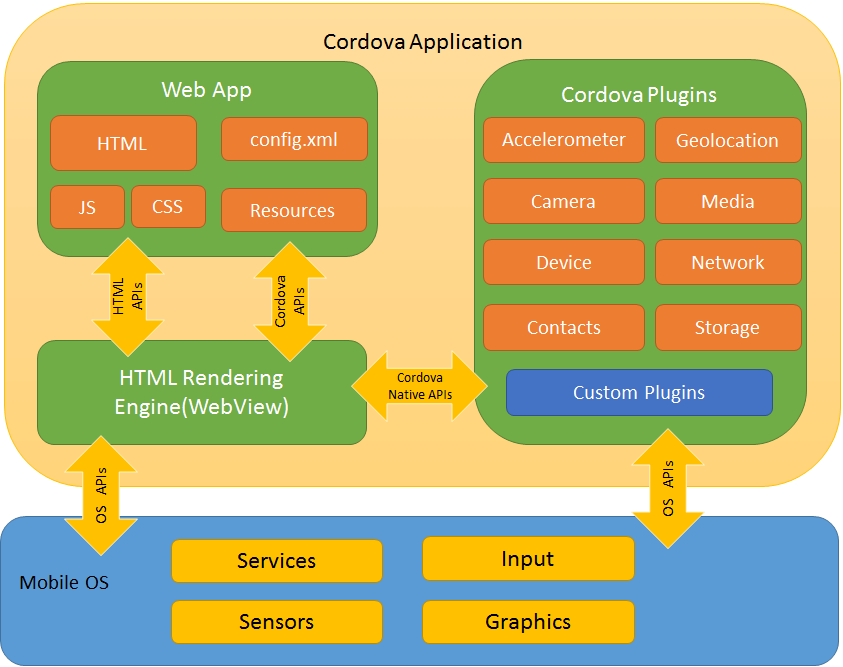
\includegraphics[width=83.82mm,height=66.3mm]{msc-img3.png}
\end{figure}
Kao što se na slici vidi, Apache Cordova implementira WebView komponentu
koja služi za prikaz korisničkog interfejsa, kao i posebne interfejse
kojima se pristupa komponentama mobilnog operativnog sistema na kom se
aplikacija izvršava. U gornjem desnom uglu su prikazani neki od
dodataka, a važno je napomenuti da je moguće implementirati i druge
dodatke samostalno.

Velika prednost Apache Cordova biblioteke (i drugih sličnih biblioteka)
je jednostavnost upotrebe. Ona ne zahteva nikakve posebne alate za
razvoj, dovoljno je samo poznavanje HTML/CSS/JS jezika. Takođe, moguće
je koristiti i popularne JavaScript biblioteke kao što su Angular ili
KnockoutJS koje doprinose čistoći i preglednosti koda.

\subsection[2.2. NativeScript[2{]}]{\rmfamily 2.2.
NativeScript\textsuperscript{[2]}}
\hypertarget{RefHeadingToc1171308303690}{}NativeScript je nova
biblioteka koju je razvila američka kompanija Telerik, koja se dugi niz
godina bavi razvojem izuzetno kvalitetnih grafičkih komponenti
korisničkog interfejsa (između ostalog) koje se mogu koristiti u
nekoliko programskih jezika.

NativeScript je takođe potpuno besplatna i open-source biblioteka koja
kao i Apache Cordova koristi JavaScript/HTML i CSS za pravljenje
cross-platform mobilnih aplikacija. NativeScript trenutno podržava
Android verziju 4.2 i više i iOS verziju 7.1 i više, dok je podrška za
Windows telefone u razvoju. Razvoj je moguć na bilo kojem Desktop
operativnom sistemu (Windows/Linux/OS X).

Glavna razlika i prednost NativeScript-a je što ne koristi WebView za
prikaz grafičkih komponenti u aplikacijama, već koristi nativne
komponente operativnog sistema. Takođe NativeScript pored funkcija koje
jednostavno mapiraju pozive na funkcije operativnog sistema sadrži i
funckije koje olakšavaju razvoj kao što su funkcije za prikaz poruka,
mrežnu komunikaciju i slično. Ovo omogućava programeru da može da
koristi ove funkcionalnosti bez da nužno zna kako one funkcionišu na
nivou mobilnog operativnog sistema.

NativeScript je još uvek u ranoj fazi razvoja, i ne postoji mogućnost
korišćenja ni jednog drugog jezika za razvoj osim JavaScript-a i
njegovih derivata, što je velika mana ukoliko se razvijaju
komplikovanije, enterprise aplikacije.

Ipak, ova biblioteka je za kratko vreme stekla veliku popularnost, i već
se može pronaći dosta kvalitetnih i popularnih aplikacija koje koriste
ovu biblioteku.

\begin{figure}
\centering
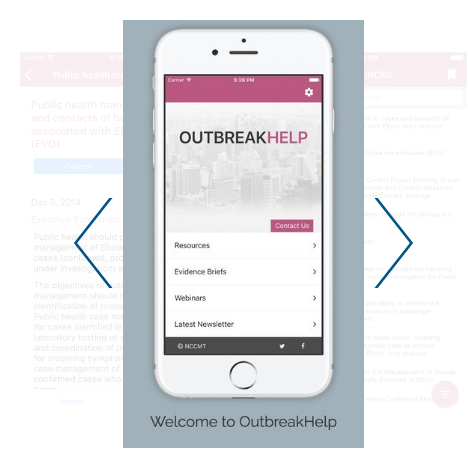
\includegraphics[width=56.55mm,height=55.1mm]{msc-img4.png}
\end{figure}
\begin{figure}
\centering
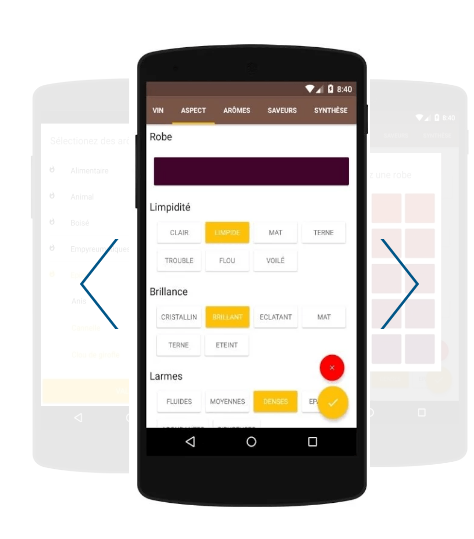
\includegraphics[width=51.01mm,height=58mm]{msc-img5.png}
\end{figure}
\begin{figure}
\centering
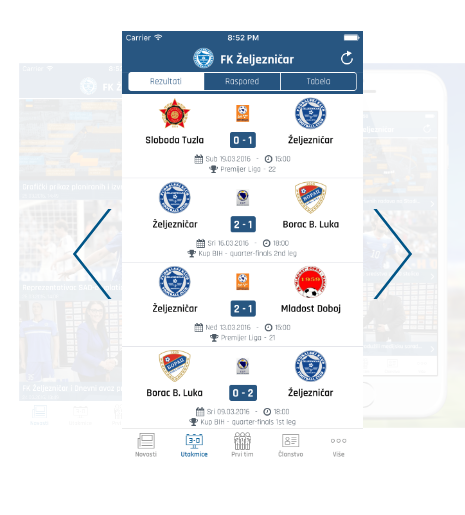
\includegraphics[width=50.39mm,height=55.81mm]{msc-img6.png}
\end{figure}
\subsection[2.3. React Native[3{]}]{\rmfamily 2.3. React
Native\textsuperscript{[3]}}
\hypertarget{RefHeadingToc871882405265}{}React Native je još jedna
biblioteka koja koristi Web tehnologije za razvoj cross-platform
mobilnih aplikacija. Razvila ju je kompanija Fejsbuk, i još uvek je u
ranoj fazi razvoja. React Native se bazira na React biblioteci koja se
koristi u razvoju Web aplikacija. Kao i NativeScript, React Native se
ne izvršava u WebView komponenti već se grafički interfejs mapira na
nativne komponente mobilnog operativnog sistema. Takođe, React Native,
kao i NativeScript, definiše svoje interfejse koji objedinjuju elemente
kao što su kontrola senzora, kamere i slično na različitim operativnim
sistema, što omogućava programeru da implementira ove delove aplikacije
bez da nužno zna kako su oni definisani u samom mobilnom operativnom
sistemu. React Native podržava iOS i Android.

Glavna prednost i novina koju React Native donosi je mogućnost da se
komponente implementiraju direktno za specifičnu mobilnu platformu u
programskim jezicima Java (za Android) i Swift ili Objective-C (za
iOS). Ovo znači da programer ima veliku fleksibilnost u poređenju sa
drugim JavaScript bibliotekama, kao i da je moguća implementacija
kritičnih komponenti u pravom nativnom smislu ukoliko postoji takva
potreba.

Mobilna aplikacija za društvenu mrežu Fejsbuk implementirana je na
upravo ovakav način.\textsuperscript{[4]}



\begin{figure}
\centering
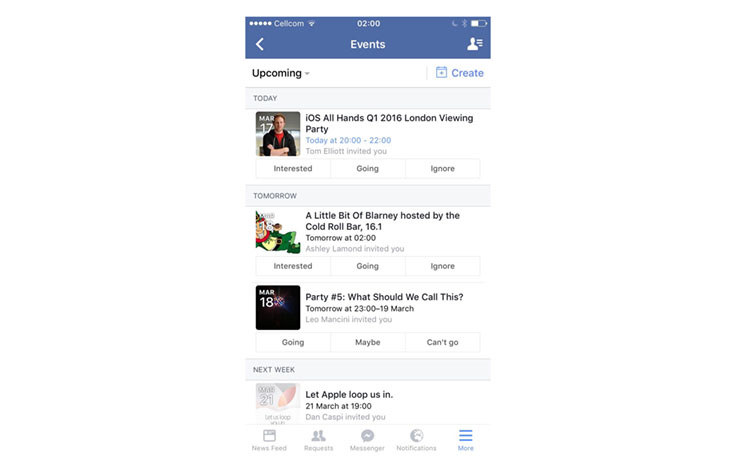
\includegraphics[width=162.56mm,height=103.8mm]{msc-img7.png}
\end{figure}
\clearpage\section[3. Native biblioteke]{\rmfamily 3. Native biblioteke}
\hypertarget{RefHeadingToc1051308303690}{}Native biblioteke za razvoj
mobilnih aplikacija su dosta komplikovanije od gore navedenih
biblioteka. One se zasnivaju na korišćenju apstrakcija i moćnih oruđa
modernih programskih jezika kao što su delegati, lambda izrazi,
generički tipovi i slično, kako bi se napravio sloj koji prevodi kod
koji programer piše u više različitih verzija koda za različite
platforme. 

Native biblioteke takođe zahtevaju često veoma zahtevne alate i
emulatore za testiranje.

U trenutku pisanja ovog rada, postoje tri dovoljno razvijene biblioteke:
CodenameOne, Kivy i Xamarin.

\subsection[3.1. CodenameOne[5{]}]{\rmfamily 3.1.
CodenameOne\textsuperscript{[5]}}
\hypertarget{RefHeadingToc1071308303690}{}CodenameOne je biblioteka koja
koristi Java kod koji se onda kompajlira i pakuje za razne mobilne
uređaje. Postoje dodaci za popularna razvojna okruženja Eclipse i
NetBeans, koji olakšavaju razvoj cross-platform nativnih aplikacija.

CodenameOne se zasniva na nekoliko koncepata:

\liststyleLii
\begin{itemize}
\item definisanje interfejsa nezavisnih od uređaja i operativnog sistema
na kojem se aplikacija izvršava
\item definisanje načina pravljenja dodataka (plugin-ova) za razna
razvojna okruženja
\item postavljanje Build servera koji kompajliraju aplikaciju
\end{itemize}
Pošto su razvojni alati za moderne mobilne platforme veliki i zahtevni,
CodenameOne pruža svoj servis za testiranje i kompajliranje aplikacija,
što znači da je moguće kompajlirati na primer za iOS bez alata
instaliranih na OS X računaru, što je inače slučaj.



\begin{figure}
\centering
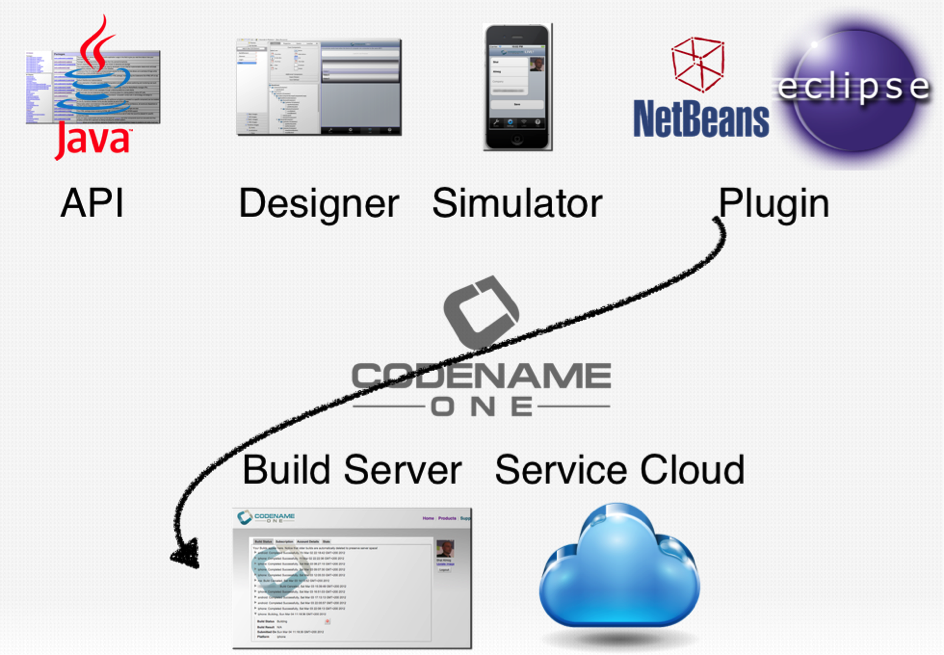
\includegraphics[width=127.04mm,height=88.14mm]{msc-img8.png}
\end{figure}
\clearpage
CodenameOne je zreo i relativno popularan projekat. Takođe je potpuno
besplatan i open-source. Međutim, pošto se kompajliranje vrši na
udaljenim serverima, potrebno je platiti mesečnu pretplatu za njihovo
korišćenje. Instalacija lokalnog build servera u trenutku pisanja ovog
rada koštala bi preko 20000 dolara. Ovaj podatak, i činjenica da je
razvoj CodenameOne projekta veoma usporen i daleko manje aktivan nego
pre, odvratilo je autora ovog rada od korišćenja.

\subsection[3.2. Kivy[6{]}]{\rmfamily 3.2. Kivy\textsuperscript{[6]}}
\hypertarget{RefHeadingToc1091308303690}{}Kivy je potpuno besplatni,
open-source alat koji omogućava programeru da pravi cross-platform
nativne aplikacije u programskom jeziku Python. Kivy se takođe može
koristiti i za razvoj Desktop aplikacija što je velika prednost u
odnosu na sve do sada navedene biblioteke. Podržava Windows, Linux, OS
X, Android i iOS. Apsolutno isti kod se može izvršavati na bilo kojoj
od navedenih platformi. Takođe, Kivy ima podršku i za grafički
intezivne aplikacije što znači da se uz pomoć ove biblioteke čak mogu
praviti i igrice. 

Kivy ne koristi nativne grafičke komponente, već definiše svoje.
Grafički interfejs je takođe moguće definisati posebnim Kv jezikom.
Python kod se prevodi u C kod (CPython) koji se zatim koristi na
mobilnim uređajima.



\begin{figure}
\centering
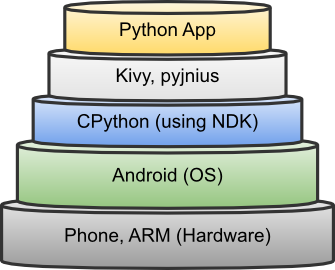
\includegraphics[width=60.59mm,height=48.84mm]{msc-img9.png}
\end{figure}
Od svog začeća 2011. godine do danas, Kivy je u veoma aktivnom razvoju i
sada je već stabilna i zrela platforma za rad koju koriste mnoge
aplikacije kako desktop tako i mobilne. Kivy razvija neprofitna
organizacija Kivy Organization koju čine veoma iskusni Python
programeri.

Autor ovog rada ima iskustva sa Python programskim jezikom i sa Kivy
bibliotekom ali se ipak odlučio na korišćenje druge biblioteke zbog
daleko bolje razvijenosti, daleko većih mogućnosti i daleko većih
performansi.

\clearpage\subsection[3.3. Xamarin[7{]}]{\rmfamily 3.3.
Xamarin\textsuperscript{[7]}}
\hypertarget{RefHeadingToc1111308303690}{}Xamarin je (od nedavno)
besplatna i open-source platforma za razvoj mobilnih aplikacija,
vlasništvo kompanije Microsoft. Xamarin koristi nativne komponente
mobilnih operativnih sistema, nativne sistemske pozive mapira u svoje
interfejse, i postiže izuzetno visoke performanse na svim platformama.

Xamarin takođe podržava integraciju sa bibliotekama za razvoj moblnih
igara (Unity). 

Xamarin koristi programski jezik C\# za kod i markup jezik XAML za
definisanje korisničkog interfejsa. Korisnički interfejs je takođe
moguće definisati uz pomoć C\#. 

Xamarin projekte odlikuje izuzetno visok stepen deljenog koda.



\begin{figure}
\centering
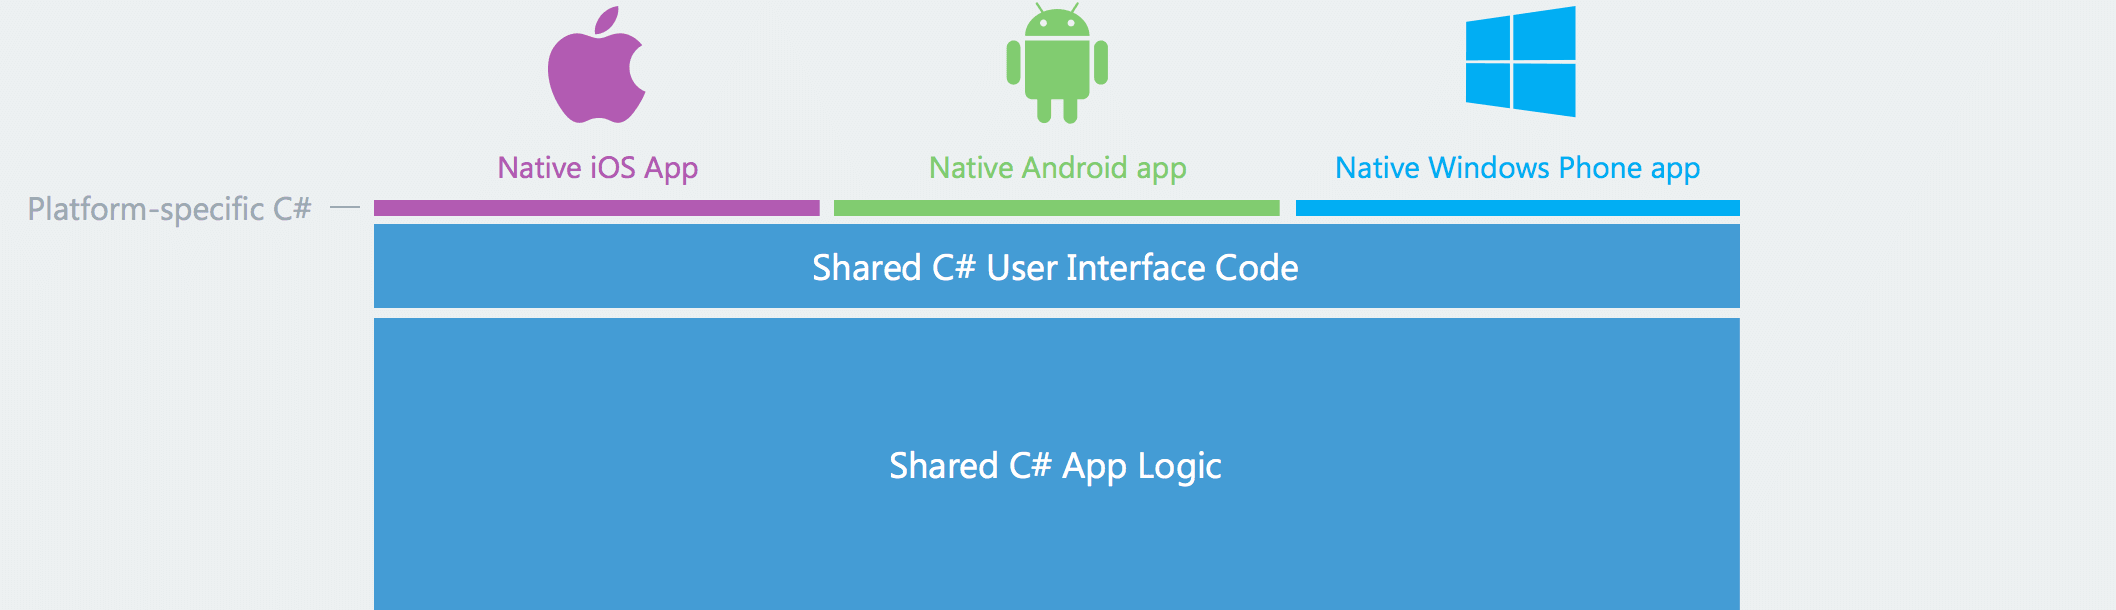
\includegraphics[width=170mm,height=49mm]{msc-img10.png}
\end{figure}
Ovo je postignuto korišćenjem veoma velikog niza modernih osobina
programskog jezika C\# (koji je odabran baš iz tog razloga) kao što su
kompleksne strukture, asinhrone funkcije, lambda izrazi, delegati i
slično.

Xamarin trenutno podržava Android (mobilni telefoni, tableti, pametni
satovi), iOS (telefoni, tableti), Windows (Universal Windows Platform –
desktop i mobilne aplikacije) a dostupna razvojna okruženja su Visual
Studio (na Windows operativnom sistemu) i Xamarin Studio (na OS X
operativnom sistemu). Razvojno okruženje za Linux (MonoDevelop)
postoji, ali nije u potpunosti podržano. 

Za kompajliranje Xamarin aplikacija za iOS potreban je računar sa OS X
operativnim sistemom. Xamarin tim je razvio alate koji olakšavaju
proces slanja kompajliranja i simuliranja izvršavanja aplikacije, tako
da OS X računar može biti negde daleko na mreži, i programer ne mora da
ima fizički pristup istom.

Xamarin.Forms je novi, podrazumevani način razvoja grafičkih okruženja u
Xamarin biblioteci. Definišu se XAML fajlovi (XAML je markup jezik
sličan XML-u, više detalja u daljem tekstu) koji se zatim transformišu
u nativne komponente na svim platformama za koje se kompajlira.

Xamarin projekat koristi Mono (open-source implementaciju .NET
Framework-a) za izvršavanje C\# kod-a na Android i iOS operativnim
sistemima. To znači da nema prevođenja koda koji programer direktno
piše u različit kod za različite platforme, već da se zaista isti C\#
kod izvršava na više različitih platformi.

Postoje dva načina postizanja deljivosti koda u definiciji samog
projekta:

\liststyleLiii
\begin{enumerate}
\item korišćenjem takozvanih Shared projekata
\item i korišćenjem PCL (Portable Class Library) projekata
\end{enumerate}
Način dalje korišćen u ovom radu (i preporučeni način) je korišćenjem
PCL projekata prikazanim na sledećoj slici.


\bigskip



\begin{figure}
\centering
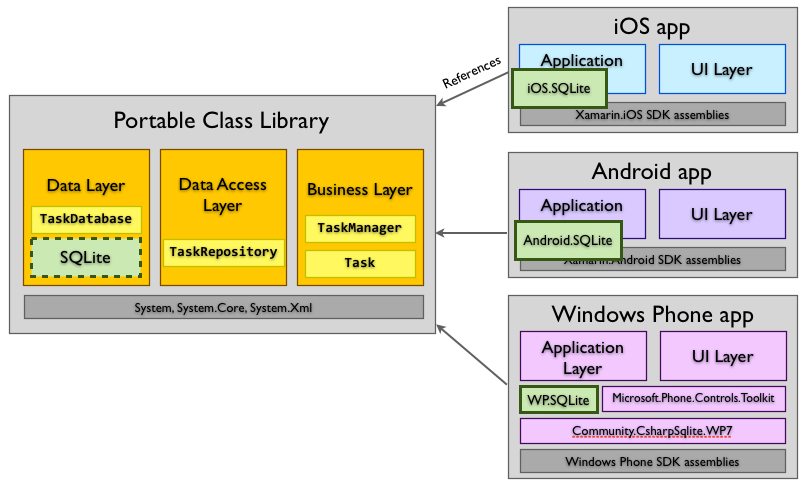
\includegraphics[width=135.2mm,height=81.72mm]{msc-img11.png}
\end{figure}
Ovakav koncept izrade aplikacija je veoma interesantan. Naime, programer
piše klasičnu .NET C\# biblioteku koristeći Xamarin interfejse koju
zatim drugi projekti (za specifične platforme) koriste. Dakle,
programer nema nikakvu potrebu na menja projekte za specifične
platforme, postoji samo jednostavna zavisnost između projekta za
specifičnu platformu i PCL projekta.

Naravno, postoji mogućnost izmena projekata za različite platforme, čak
i predefinisani načini u Xamarin biblioteci uz čiju pomoć je ovaj
proces znatno olakšan.

Xamarin biblioteka ima odličnu dokumentaciju i veoma veliku podršku
pošto je mnogo programera koristi. Iako je razvojno okruženje glomazno,
stabilnost, podrška za statički pisan jezik – C\#, performanse i
mogućnosti biblioteke bile su presudan faktor u odluci autora ovog rada
koju će biblioteku koristiti za razvoj aplikacije opisanu u ovom radu.

Za implementaciju aplikacije koja je prikazana u ovom radu i čija je
svrha da prikaže mogućnosti Xamarin biblioteke, kao i da prikaže neke
koncepte koje je neophodno koristiti u razvoju cross-platform native
mobilnih aplikacija korišćena je Xamarin biblioteka, Xamarin.Forms
biblioteka za razvoj grafičkog interfejsa, programski jezik C\# 6 i
razvojno okruženje Microsoft Visual Studio 2015.

Sav kod ovde prikazane aplikacije dostupan je na
\ \texttt{\textcolor[rgb]{0.0,0.4,0.8}{http://github.com/nmilosev/PMF}}\texttt{\textcolor[rgb]{0.4,0.6,0.6}{
}}

\clearpage\section[4. Motivacija za ovakav način razvoja mobilnih
aplikacija]{\rmfamily 4. Motivacija za ovakav način razvoja mobilnih
aplikacija}
\hypertarget{RefHeadingToc4171813786090}{}Važno je napomenuti koje su
prednosti razvoja hibridnih tj. cross-platform nativnh mobilnih
aplikacija, u poređenju sa razvijanjem posebnih aplikacija za sve
platforme u za to predviđenim alatima.

Prva prednost je očigledno, deljenje koda. Ukoliko bismo razvijali
aplikaciju za tri ovde navedene mobilne platforme na tradicionalan
način, tj. posebno za svaku platformu, morali bismo tri puta da pišemo
kod za svaku funkcionalnost. Takođe, morali bismo da koristimo tri
različita programska jezika, što je druga prednost kod korišćenja
biblioteke kao što je Xamarin – koristi se samo jedan programski jezik.
Treća prednost je sam rad sa interfejsima aplikacije. Biblioteke kao
što su Xamarin pružaju jedinstveni pristup mogućnostima uređaj za koji
se razvija tako što definišu jedan interfejs za pristupanje nekoj
komponenti (npr. Kompasu) čija implementacija zavisi od platforme za
koju se kompajlira aplikacija. Ukoliko bismo se odlučili da našu
aplikaciju razvijamo na tradicionalan način – morali bismo da se
upoznamo sa definicijom biblioteke za kompas (u ovom slučaju) za sve
tri različite mobilne platforme – što nam oduzima dodatno vreme.
Prednosti ima još, ovo su samo neke – najvažnije.

S druge strane, ovakav pristup razvoju ima i mana:

\liststyleLiv
\begin{itemize}
\item razvojno okruženje je veoma glomazno pošto mora da ima mogućnosti
kompajliranja za mnogo različitih platformi
\item interfejsi koje definišu biblioteke za cross-platform razvoj često
kasne za nativnim bibliotekama mobilnih operativnih sistema, što znači
da nekada može proći dosta vremena od uvođenja nove opcije operativnog
sistema do mogućnosti upotrebe te opcije u samoj biblioteci
\item gubi se potpuna kontrola nad kompajliranim kodom što može dovesti
do gubitka performansi
\item pošto se biblioteka mora spakovati u paket mobilne aplikacije,
često taj paket bude dosta veći u poređenju sa istom aplikacijom
napisanom na tradicionalan način, što može odvratiti korisnike od
preuzimanja
\item vreme kompajliranja je često duže
\item iako je nivo apstrakcije veoma veliki često je potrebno znanje
detalja implementacije specifične platforme za koju se razvija
\end{itemize}
Ipak, i pored ovih mana, u trenutku pisanja ovog rada dosta biblioteka
za cross-platform mobilne aplikacije se aktivno razvija što svedoči da
je sve veći broj programera koji se odlučuju na ovakav pristup.

\section[5. Kratka istorija Xamarin biblioteke]{5. Kratka istorija
Xamarin biblioteke}
\hypertarget{RefHeadingToc4191813786090}{}Kada je u junu 2000. godine
kompanija Microsoft objavila prvu verziju .NET framework-a nekoliko
programera je počelo na razvoju implementacije koja bi radila na Linux
operativnom sistemu. Projekat je nazvan Mono\textsuperscript{[8]} i
zvanično je objavljen 19. jula 2001. godine. Mono projekat je kasnije
bio razvijan od strane Novell i Attachmate kao delimično komercijalni
alat, koje su 2011. godine napustile projekat.

U maju 2011. godine Miguel de Icaza, glavni Mono programer i osnivač
projekta je osnovao novu kompaniju Xamarin i objavio da ponovo preuzima
održavanje Mono projekta. Takođe je naglašeno da je fokus nove
kompanije na mobilnim platformama. U tom trenutku biblioteke za razvoj
Android i iOS aplikacija su se zvale MonoAndroid i MonoTouch.

Veliki napredak u razvoju i verziju 2.0 Xamarin objavljuje u februaru
2013. godine. U isto vreme pojavljuje se i razvojno okruženje Xamarin
Studio (zasnovano na MonoDevelop razvojnom okruženju) kao i svi
potrebni alati za razvoj Android i iOS aplikacija u razvojnom okruženju
Microsoft Visual Studio. 

U sledećem periodu broj programera koji koriste Xamarin biblioteku
znatno raste i biblioteka postaje sve zrelija i moćnija.

U verziji 3 koja je objavljena u maju 2014. godine pojavljuje se i
biblioteka Xamarin.Forms za definisanje grafičkog interfejsa aplikacije
na jedinstven način za sve platforme.

Jedan od glavnih problema Xamarin biblioteke bila je cena. Cena
korišćenja ove biblioteke bila je oko \$3000 godišnje po programeru,
što mnogi programeri nisu mogli da opravdaju pogotovo što su čak i u
tom trenutku postojala alternativna besplatna open-source rešenja.

U februaru 2016. godine u zvaničnom objavljenju navodi se da je
kompanija Microsoft novi vlasnik kompanije Xamarin i svih prava na
Xamarin biblioteke. Tačan iznos za koji je Microsoft kupio kompaniju
Xamarin nije poznat.

Ubrzo nakon toga na Microsoft Build 2016 konferenciji, Microsoft
objavljuje da će cela Xamarin biblioteka biti potpuno besplatna za
korišćenje i u potpunosti open-source pod MIT licencom. Takođe, Mono
(open-source implementacija .NET framework-a) koji je takođe bio
vlasništvo kompanije Xamarin, postaje ponovo u potpunosti open-source
posle skoro 20 godina.

U trenutku pisanja ovog rada Xamarin je u potpuno besplatan i
open-source alat koji se lako može preuzeti sa sajta
\texttt{\textcolor[rgb]{0.0,0.4,0.8}{http://xamarin.com}} ili uz
besplatno razvojno okruženje Microsoft Visual Studio 2015 Community

Aplikacije pisane korišćenjem Xamarin biblioteke mogu se bez naknade
objavljivati na servisima kao što su Google Play Store, Apple AppStore
ili Windows Store.

\clearpage\section[6. Xamarin.Forms[9{]} biblioteka]{\rmfamily 6.
Xamarin.Forms\textsuperscript{[9]} biblioteka}
\hypertarget{RefHeadingToc10541394079323}{}Ukoliko bi se Xamarin
biblioteka koristila samostalno, korisnički interfejs aplikacije morao
bi biti implementiran za svaku platformu posebno. Rešenje ovog problema
je upotreba Xamarin.Forms biblioteke.

Xamarin.Forms biblioteka, koja je korišćena u izradi aplikacije za
studentske servise, je skup komponenti tj. mapiranja do nativnih
komponenti na svakoj od podržanih platformi. Korišćenjem Xamarin.Forms
komponenti, moguće je implementirati korisnički interfejs za sve
odvojene platforme na jedinstveni način.

Xamarin.Forms biblioteka definiše komponente koje se pri kompajliranju
prevode u nativne komponente. Na primer,
\texttt{\textcolor[rgb]{0.0,0.4,0.8}{Entry}} komponenta iz ove
biblioteke će postati \texttt{\textcolor[rgb]{0.0,0.4,0.8}{UITextView}}
na iOS platformi, \texttt{\textcolor[rgb]{0.0,0.4,0.8}{EditText}} na
Android platformi i \texttt{\textcolor[rgb]{0.0,0.4,0.8}{TextBox}} na
Windows platformi kao što je prikazano na sledećoj slici: 



\begin{figure}
\centering
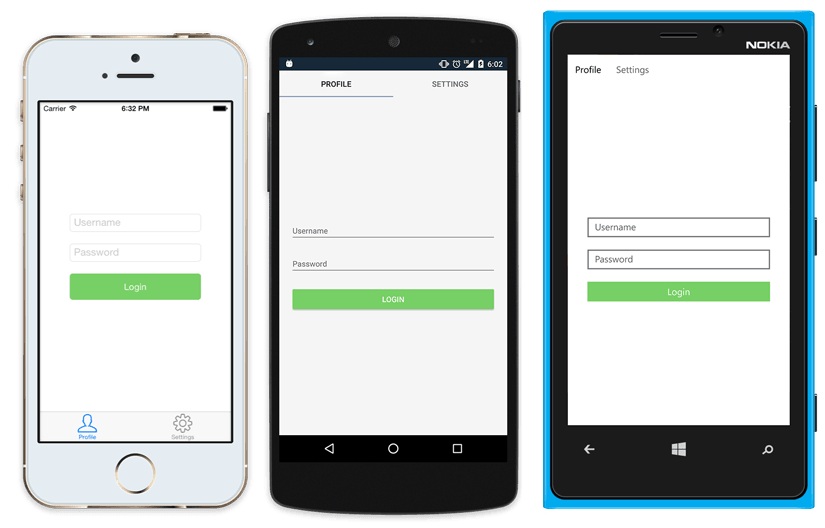
\includegraphics[width=142.12mm,height=90.95mm]{msc-img12.png}
\end{figure}
Xamarin.Forms biblioteka je trenutno u razvoju, međutim zbog lakoće
upotrebe, sve više programera se odlučuje da je koristi za nove
projekte. Takođe, Xamarin.Forms biblioteka je trenutno veoma aktivno
razvijana od strane Xamarin tima u nadi da će u budućnosti postati
standard.

Osim predefinisanih komponenti, Xamarin.Forms biblioteka omogućava
programerima da pišu i svoje komponente koje će raditi na svim
podržanim platformama. Pored ovoga, moguće je čak i ubacivanje
specifičnih nativnih komponenti u Xamarin.Forms interfejse ukoliko
postoji takva potreba.

Većina Xamarin.Forms komponenti je dizajnirana sa MVVM paternom u vidu,
tako da skoro sve podržavaju Data Binding na nekim svojim poljima.

Takođe, Xamarin.Forms biblioteka definiše skup interfejsa za pristup
servisima operativnih sistema kao što su prikazivanje notifikacija,
upotreba kamere i slično.

Glavna prednost Xamarin.Forms biblioteke je visok nivo apstrakcije.
Programer ne mora da zna detalje implementacije komponenti na
različitim platformama i komponente zaista rade isto na svim
platformama.

Najinteresantniji aspekt Xamarin.Forms biblioteke je što omogućava
definiciju korisničkog interfejsa u markup jeziku XAML.

\subsection[6.2. XAML[10{]}]{6.2. XAML\textsuperscript{[10]}}
\hypertarget{RefHeadingToc1452255603686}{}XAML, skraćeno eXtensible
Application Markup Language, omogućava programerima da definišu
korisnički interfejs i u potpunosti ga izdvoje od ostatka aplikacije.
XAML je veoma moćan alat, pogotovo kad se koristi za implementaciju
MVVM dizajn paterna.

XAML je jezik zasnovan na XML jeziku koji je razvila kompanija Microsoft
specifično za konstrukciju bogatih i komplikovanih korisničkih
interfejsa. Osim u Xamarin.Forms biblioteci, XAML se koristi i za
Desktop aplikacije (Windows Presentation Framework), Silverlight
aplikacije i nove univerzalne Windows aplikacije.

XAML jezik ima mobućnosti kao što su instanciranje objekata, podešavanje
njihovih parametara i laku manipulaciju sa parent-child odnosima.

Prednosti definisanja korisničkog interfejsa u XAML jeziku u poređenju
sa definisanjem u čistom C\# su mnoge:

\liststyleLv
\begin{itemize}
\item XAML je mnogo lakši za razumevanje i izuzetno pregledan jezik
\item pošto je baziran na XML jeziku, veoma je laka manipulacija sa
kolekcijama, odnosima parent-child i slično
\item XAML jezik je podržan od mnogih vizuelnih editora koji odmah mogu
da prikažu kako će korisnički interfejs izgledati, često i bez
kompajliranja
\end{itemize}
Naravno, postoje i neki nedostaci:

\liststyleLvi
\begin{itemize}
\item XAML ne sme sadržati kod poslovne logike, već se oslanja na
event-ove ili komande napisane u C\# klasama
\item XAML ne sadrži koncept petlji, već se prikazivanje kolekcija svodi
na kombinaciju Data Binding-a i definisanja mustre (template) po kojoj
će jedan objekat kolekcije biti prikazan
\item XAML ne sadrži koncept naredbi grananja, ovo se takođe postiže uz
pomoć Data Binding-a
\item XAML ne zna kako da instancira klasu koja nema konstruktor bez
parametara
\item XAML nema mogućnost pozivanja metoda, već se ponovo, oslanja na
Data Binding
\end{itemize}
U trenutku pisanja ovog rada vizualni dizajner za XAML kod u
Xamarin.Forms biblioteci je u ranoj fazi razvoja. Jedina „pomoć“ je
tekstualni dizajner u Visual Studio alatu koji pomaže oko sintakse i
definicije novih komponenti.

Svaki XAML fajl ima ekstenziju
\texttt{\textcolor[rgb]{0.0,0.4,0.8}{.xaml}} i radi zajedno sa jednom
C\# klasom koja u ovom slučaju ima isto ime kao XAML fajl i ekstenziju
\texttt{\textcolor[rgb]{0.0,0.4,0.8}{.xaml.cs}}

Na primer, jedna od stranica iz aplikacije za studentske servise:

i njena prateća C\# klasa:

\begin{figure}
\centering
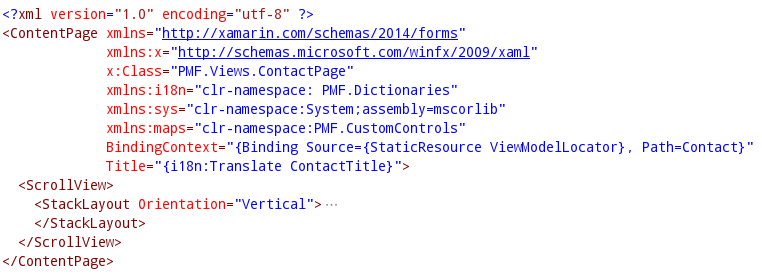
\includegraphics[width=168.08mm,height=60.08mm]{msc-img13.png}
\end{figure}


\begin{figure}
\centering
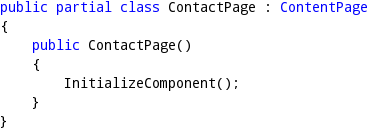
\includegraphics[width=82.16mm,height=28.93mm]{msc-img14.png}
\end{figure}
XAML kod i C\# kod zapravo predstavljaju jednu klasu koja je podeljena u
dva fajla – ovo je moguće korišćenjem ključne reči partial u C\# kodu.

U XAML kodu neophodno je navesti u potpunosti kvalifikovano ime klase, i
XAML elemenat koji navodi ovo mora biti istog tipa kao i nadklasa
navedene C\# klase.

U konstruktoru C\# klase pozivom metoda
\texttt{\textcolor[rgb]{0.0,0.4,0.8}{InitializeComponent}} XAML fajl će
se parsirati i napraviće se sva polja i objekti klase koji onda dalje
mogu da se koriste.

C\# klasa se u ovom slučaju često naziva code-behind klasa. U
implementaciji MVVM dizajn paterna, jedno od pravila je da se kod iz
code-behind klasa u potpunosti eliminiše. Razlog ovome je što u ovom
slučaju, \texttt{\textcolor[rgb]{0.0,0.4,0.8}{ContactPage}} klasa
definiše isključivo korisnički interfejs a ne logiku same aplikacije
koju bi trebalo da definiše odgovarajuća ViewModel klasa.

MVVM dizajn patern će detaljnije biti opisan u daljem tekstu.

\clearpage\section[7. Aplikacija za studentske servise]{\rmfamily 7.
Aplikacija za studentske servise}
\hypertarget{RefHeadingToc4211813786090}{}Cilj ovog rada je da prikaže
razvoj jedne moderne cross-platform nativne mobilne aplikacije. Za ovu
svrhu osmišljena je mobilna aplikacija za studentske servise
Prirodno-matematičkog fakulteta u Novom Sadu. Aplikacija ima sledeće
mogućnosti i funkcionalnosti:

\liststyleLvii
\begin{itemize}
\item prikaz vesti sa predviđenog web servisa
\item prikaz rasporeda časova po departmanima/smerovima/studijskim
programima/ semestrima – po danima
\item detaljni prikaz studijskih programa osnovnih, master i doktorskih
studija
\item detaljni prikaz detalja studijskih programa i njihovih obaveznih i
izbornih predmeta i predmetnih nastavnika
\item pomoćnik pri odabiru izbornih i obaveznih predmeta kako bi se
uklopili u prethodno određeni broj ESPB (eng. ECST)
\item detaljan prikaz detalja i kontaktnih informacija predmetnih
nastavnika i asistenata
\item prikaz čestih pitanja i odgovora sa predviđenog web servisa
\item automatski kontakt studentske službe iz aplikacije sa mogućnosti
navigacije do Prirodno-matematičkog fakulteta pomoću eksterne
aplikacije (Google Maps na Android platformi, Apple Maps na iOS
platformi, Bing Maps na Windows platformi)
\end{itemize}

\bigskip

\clearpage
Na sledećem Use Case UML dijagramu vide se mogućnosti aplikacije:

\subsection[]{\rmfamily }
\begin{figure}
\centering
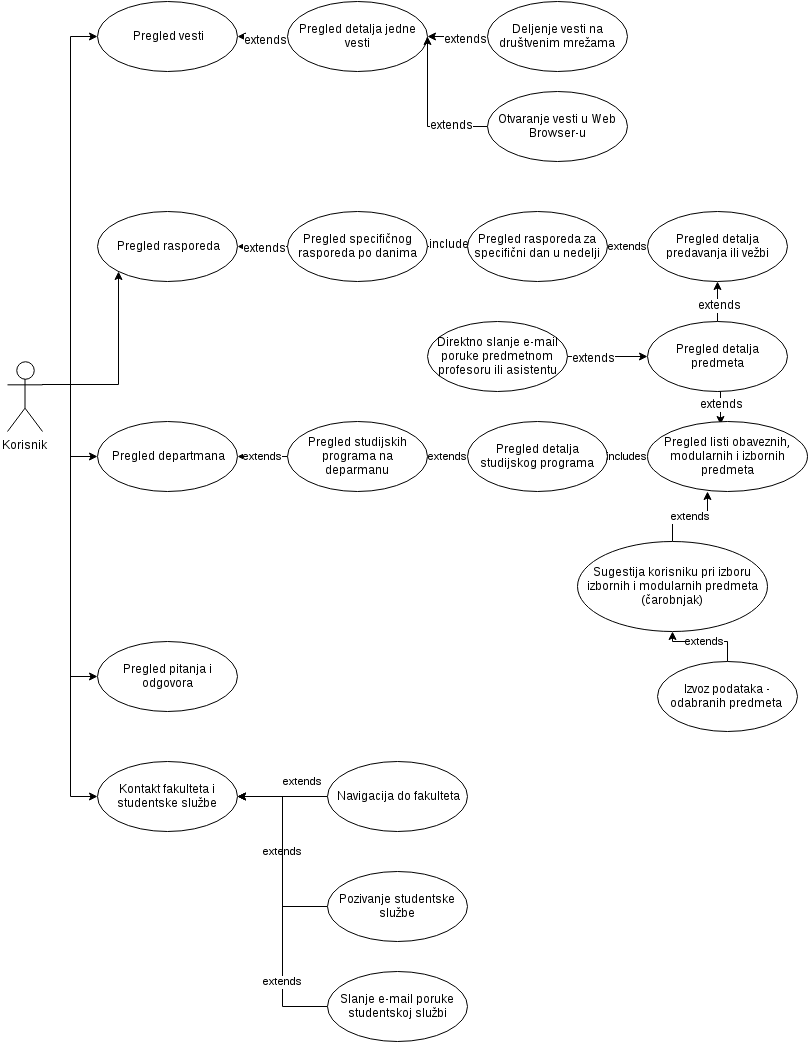
\includegraphics[width=163.62mm,height=210.93mm]{msc-img15.png}
\end{figure}

\bigskip

Korisnički interfejs aplikacije – nije sve prikazano (sve tri platforme
– Andorid 6.0 telefon, iOS 9 telefon, Windows 10 tablet):


\bigskip

Početna strana:

\begin{figure}
\centering
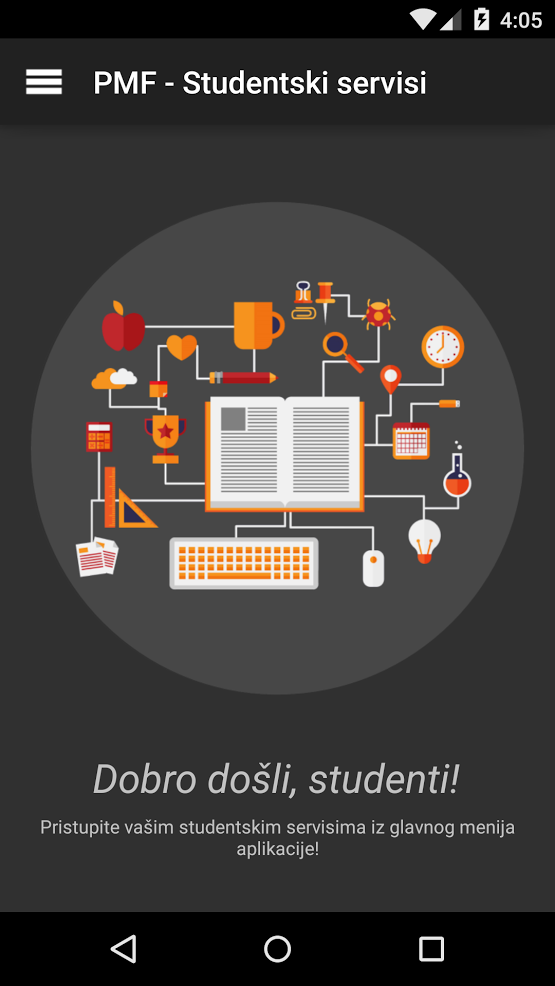
\includegraphics[width=36.21mm,height=64.29mm]{msc-img16.png}
\end{figure}
\begin{figure}
\centering

\includegraphics[width=37.5mm,height=66.68mm]{msc-img17.png}
\end{figure}
\begin{figure}
\centering
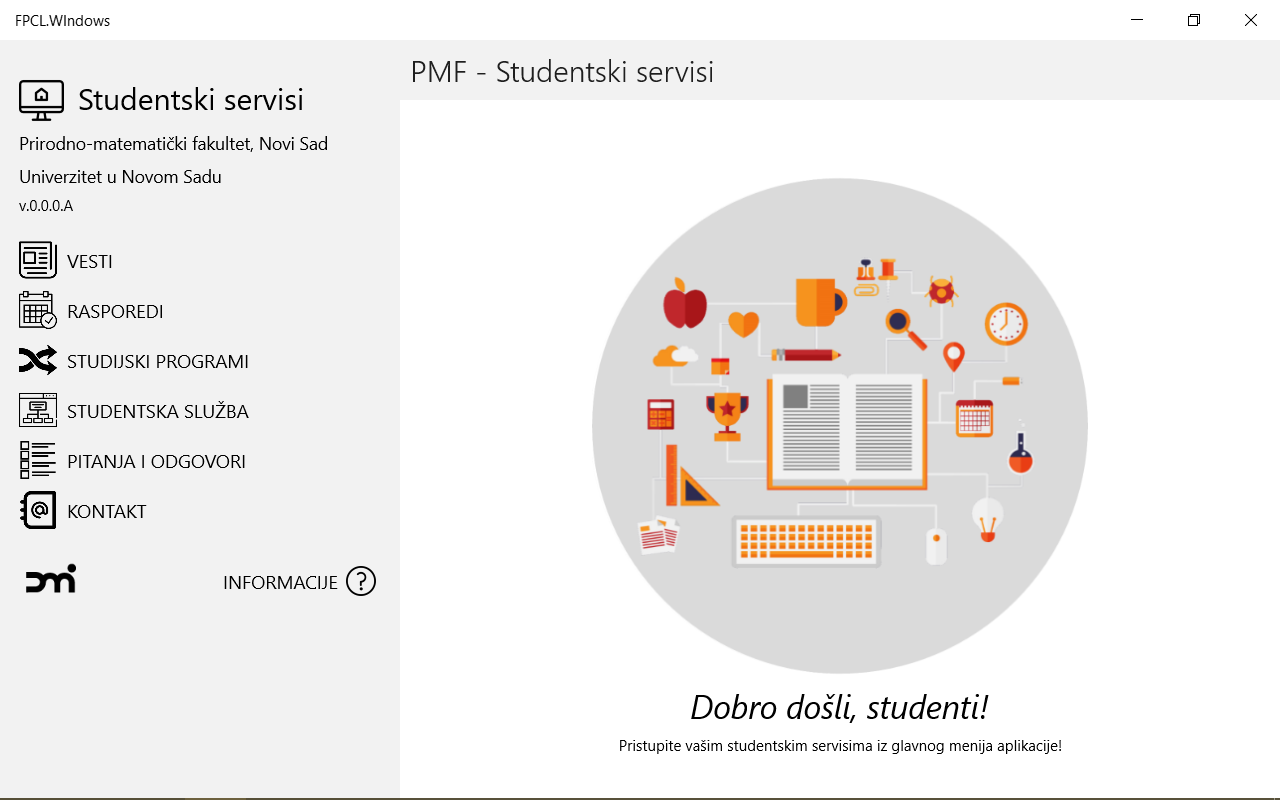
\includegraphics[width=93.35mm,height=58.33mm]{msc-img18.png}
\end{figure}

\bigskip


\bigskip



\begin{figure}
\centering
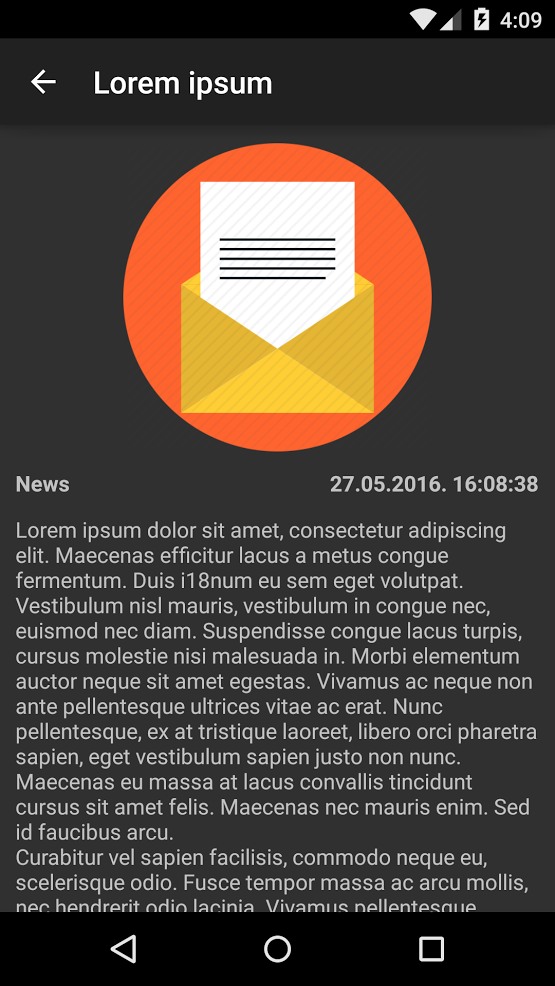
\includegraphics[width=36.76mm,height=65.3mm]{msc-img19.png}
\end{figure}
\begin{figure}
\centering
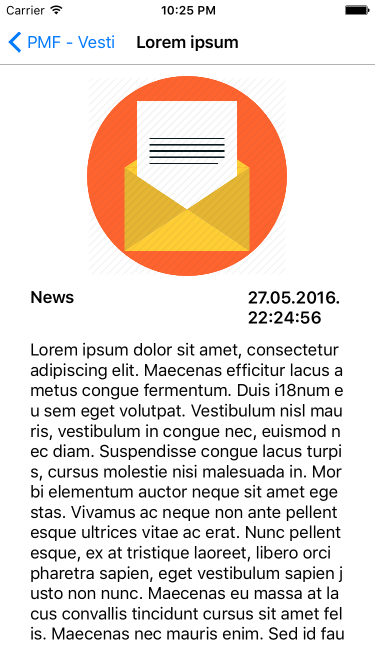
\includegraphics[width=41.08mm,height=73.06mm]{msc-img20.png}
\end{figure}
\begin{figure}
\centering
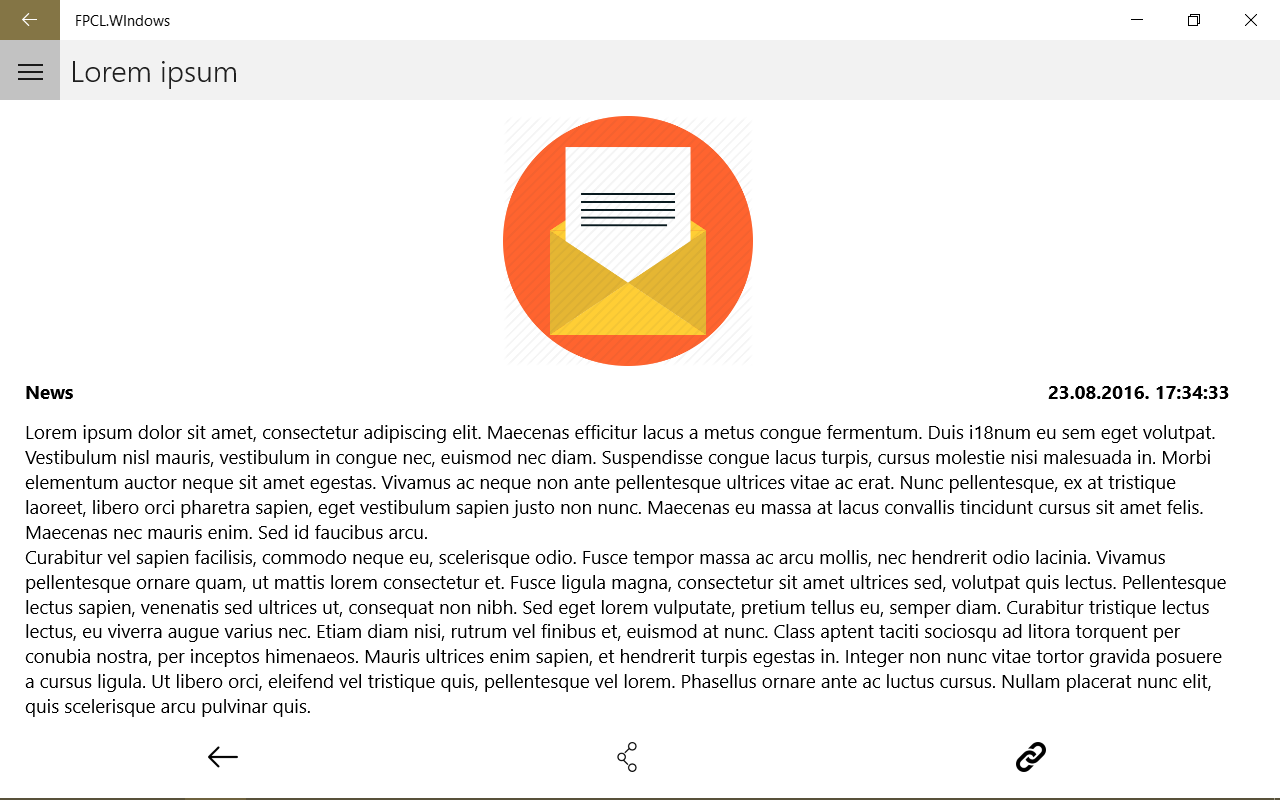
\includegraphics[width=94.37mm,height=58.97mm]{msc-img21.png}
\end{figure}
Pregled vesti:

\clearpage
Pregled detalja predmeta:



\begin{figure}
\centering

\includegraphics[width=37.66mm,height=66.97mm]{msc-img22.png}
\end{figure}
\begin{figure}
\centering

\includegraphics[width=35.1mm,height=62.32mm]{msc-img23.png}
\end{figure}
\begin{figure}
\centering
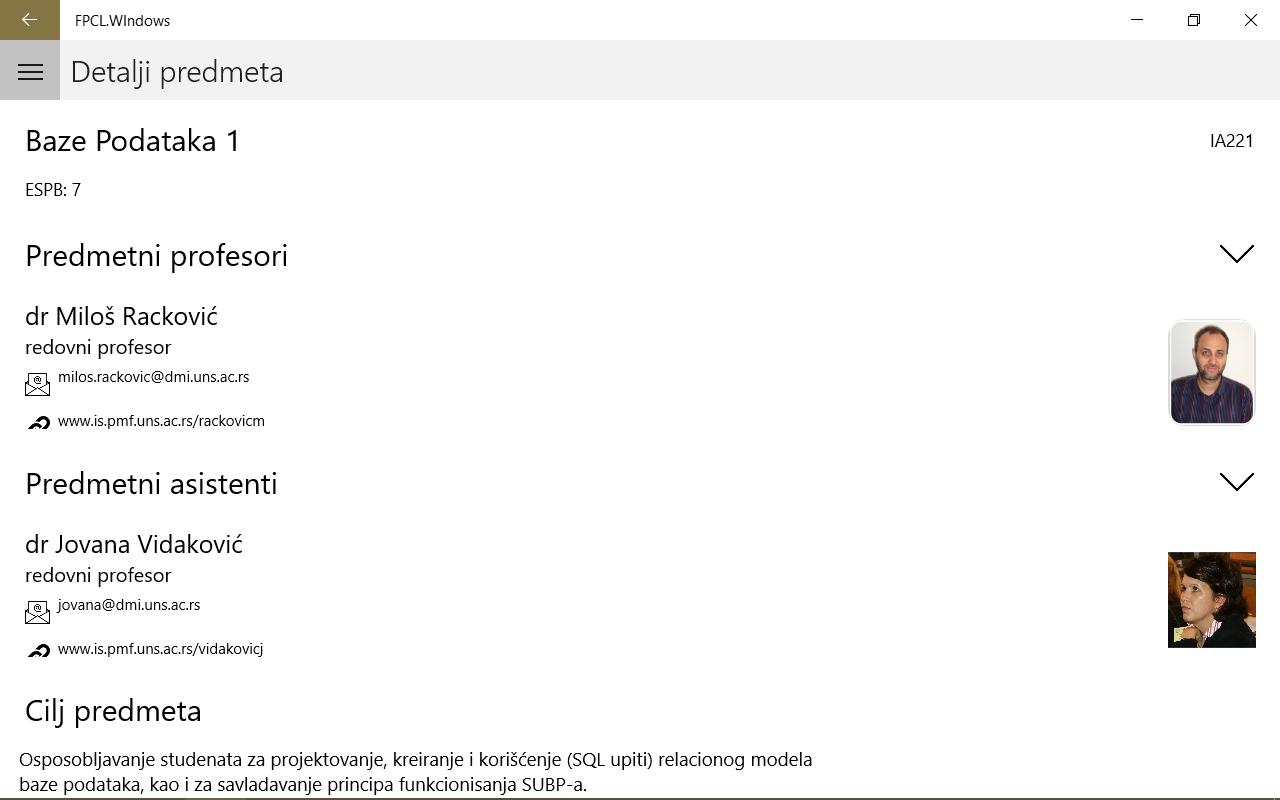
\includegraphics[width=91.93mm,height=57.45mm]{msc-img24.png}
\end{figure}
Pregled rasporeda časova:

\begin{figure}
\centering
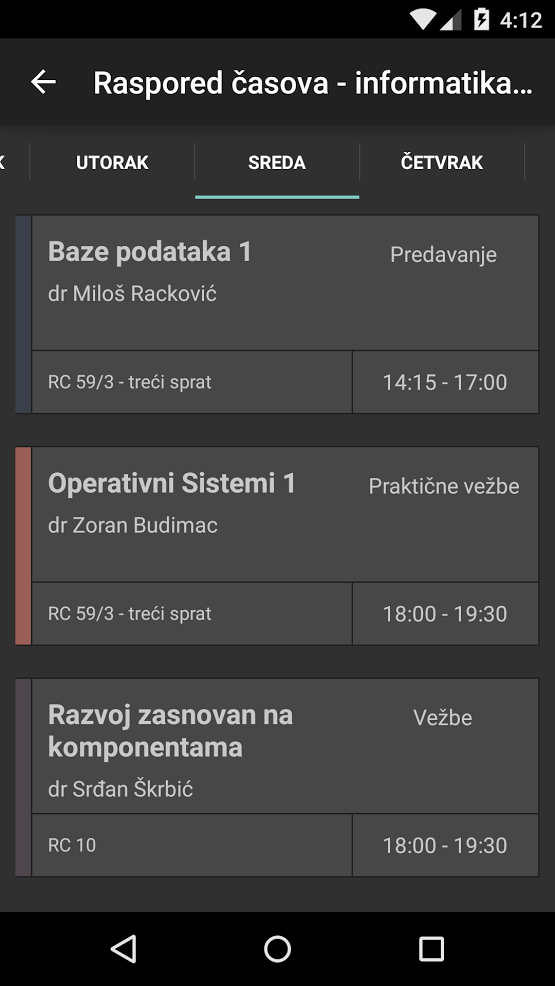
\includegraphics[width=36.02mm,height=63.98mm]{msc-img25.png}
\end{figure}
\begin{figure}
\centering

\includegraphics[width=35.14mm,height=62.42mm]{msc-img26.png}
\end{figure}
\begin{figure}
\centering
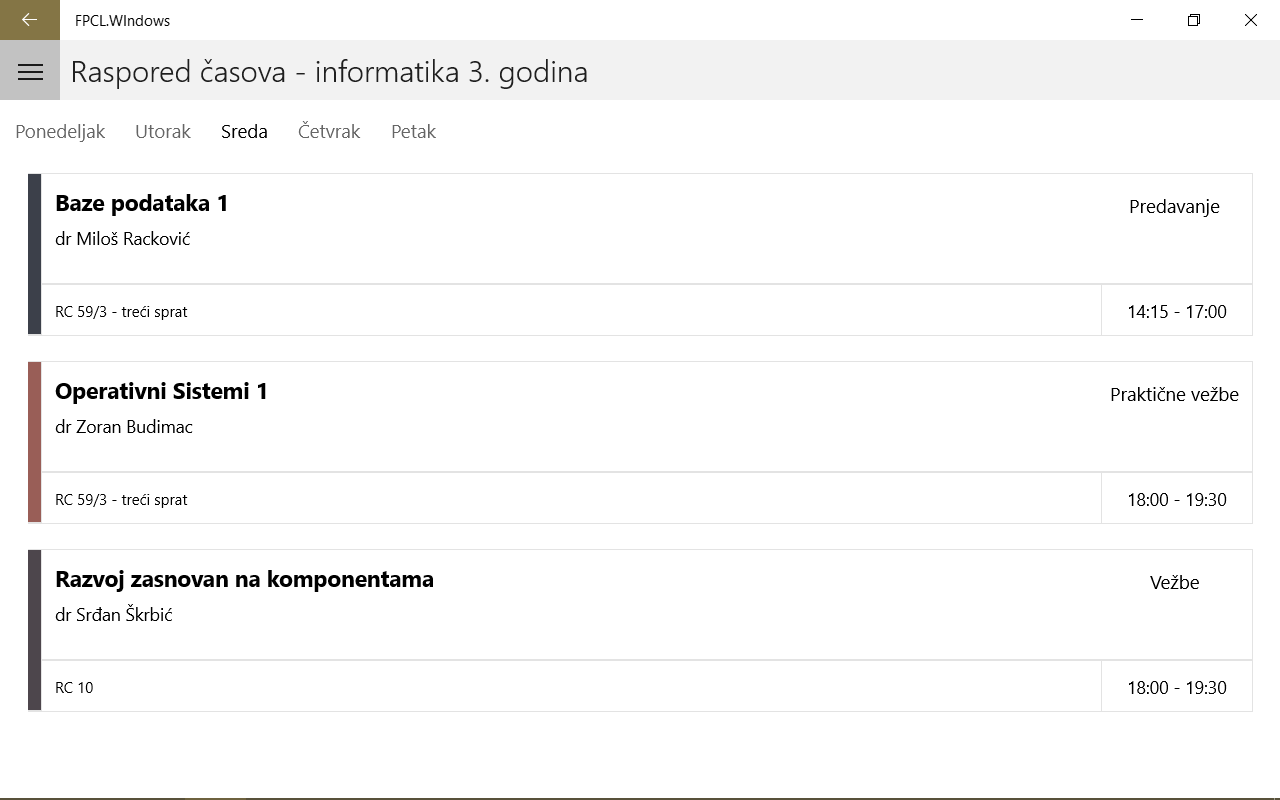
\includegraphics[width=90.1mm,height=56.3mm]{msc-img27.png}
\end{figure}


\begin{figure}
\centering
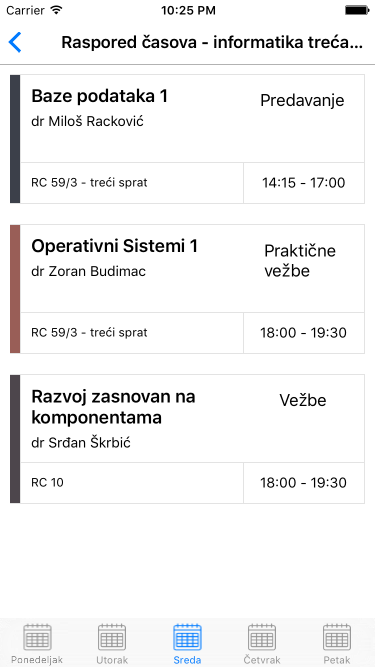
\includegraphics[width=39.92mm,height=70.96mm]{msc-img28.png}
\end{figure}
Pregled detalja aplikacije: 

\begin{figure}
\centering
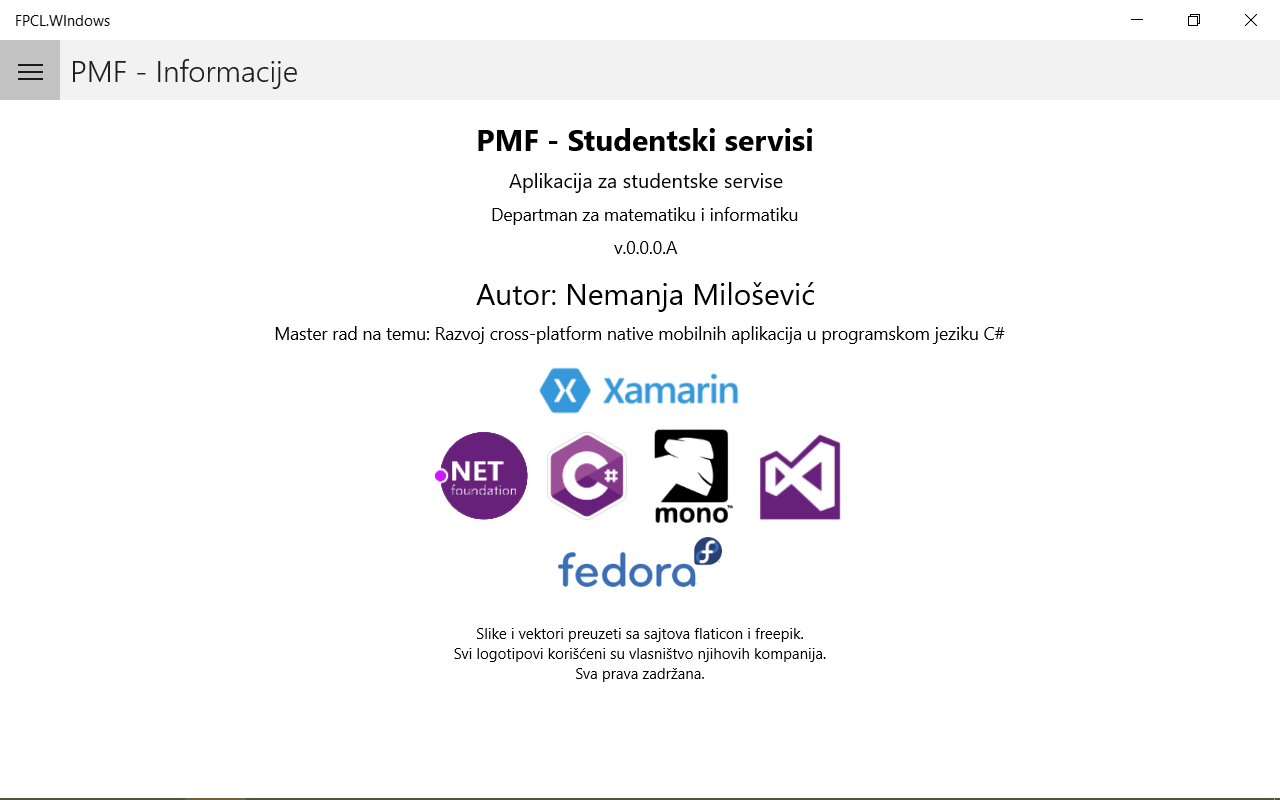
\includegraphics[width=84.75mm,height=52.97mm]{msc-img29.png}
\end{figure}
\begin{figure}
\centering

\includegraphics[width=41.65mm,height=74.07mm]{msc-img30.png}
\end{figure}
\clearpage\subsection[7.1. Korišćene tehnologije, biblioteke i dizajn
paterni]{\rmfamily 7.1. Korišćene tehnologije, biblioteke i dizajn
paterni}
\hypertarget{RefHeadingToc4231813786090}{}U ovom poglavlju biće opisane
tehnologije, open-source biblioteke i dizajn paterni koji su korišćeni
u razvoju aplikacije.

\subsubsection[7.1.1. Onion arhitektura[11{]}]{\rmfamily 7.1.1. Onion
arhitektura\textsuperscript{[11]}}
\hypertarget{RefHeadingToc4251813786090}{}

\begin{figure}
\centering
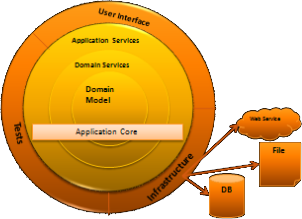
\includegraphics[width=96.84mm,height=68.53mm]{msc-img31.png}
\end{figure}
Za razvoj ovde prikazane aplikacije korišćena je Onion arhitektura.
Onion arhitektura je relativno nov pristup struktuiranju aplikacije
koji je veoma sličan tradicionalnim slojevitim aplikacijama. Ovakav
pristup odlikuje visok nivo apstrakcije a glavna razlika u odnosu na
tradicionalni slojeviti pristup je što najniži sloj aplikacije nije
sloj baze podataka kao što je često slučaju u tradicionalnom slojevitom
pristupu, već je osmišljen nov koncept najnižeg sloja koji je nazvan
jezgro (eng. Core) aplikacije. 

U ovom sloju aplikacije nalaze se klase koje opisuju tipove podataka sa
kojima aplikacija radi i svi interfejsi aplikacije, dok je baza
podataka u najvišem sloju (spoljašnjem) aplikacije i lako se može
zameniti drugom bazom podataka ili drugom vrstom servisa za
skladištenje podataka. Klase i interfejsi u ovom sloju su veoma
jednostavni, na primer, klasa koja opisuje predmetnog nastavnika ili
asistenta:



\begin{figure}
\centering
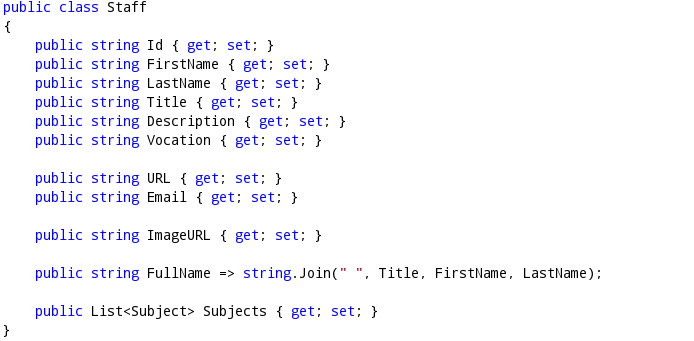
\includegraphics[width=170mm,height=83.52mm]{msc-img32.png}
\end{figure}
U ovom sloju su definisani i interfejsi aplikacije kao što je na primer
interfejs za studijske programe:


\bigskip



\begin{figure}
\centering
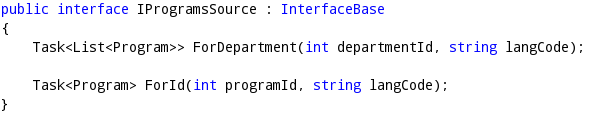
\includegraphics[width=153.21mm,height=28.82mm]{msc-img33.png}
\end{figure}
Takođe, svi interfejsi aplikacije koji rade sa podacima nasleđuju
interfejs \texttt{\textcolor[rgb]{0.0,0.4,0.8}{InterfaceBase}}:



\begin{figure}
\centering
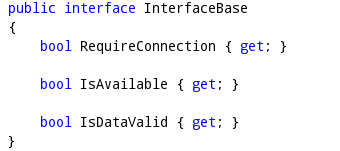
\includegraphics[width=83.7mm,height=37.17mm]{msc-img34.png}
\end{figure}
koji definiše neke zajedničke osobine kao što su da li je potrebna
internet konekcija za funkcionisanje, da li je servis dostupan, da li
su podaci trenutno u memoriji validni.

Sloj koji je oko sloja jezgra aplikacije je sloj sa servisima koji rade
nad tim podacima. Važno je napomenuti da se u ovom sloju ne nalazi
poslovna logika aplikacije već samo operacije koje rad nad običnim
(POCO – Plain Old CLR Object) objektima jezgra aplikacije i koje ne
znaju ništa o logici aplikacije. Svrha ovog sloja je da omogući
programerima još jedan stepen apstrakcije između podataka i sloja
poslovne logike.

Sloj koji je oko sloja servisa domena aplikacije je sloj sa poslovnom
logikom. U ovom sloju su implementirane operacije koje rade sa podacima
kao i sve druge operacije koje nekako imaju veza sa njima ili nekako
manipulišu podatke. 

U najvišem sloju su moduli za korisnički interfejs, bazu podataka,
testove i drugo. Svrha ovakve raspodele je da se ove komponente mogu
lako zameniti bez potrebe da se menjaju delovi iz jezgra aplikacije.

\subsection[7.2. Struktura koda aplikacije]{\rmfamily 7.2. Struktura
koda aplikacije}
\hypertarget{RefHeadingToc4271813786090}{}U ovom poglavlju biće opisana
struktura projekta aplikacije. Za ovu aplikaciju korišćen je jedan od
predviđenih načina razvoja Xamarin aplikacija kao
PCL\textsuperscript{[12]} (Portable Class Library). U ovakvom načinu,
sav deljeni kod aplikacije se kompajlira u jednoj portabilnoj
biblioteci koja se zatim koristi u projektima specifičnim za razne
platforme. Ovaj veoma interesantan pristup pisanju aplikacije kao
biblioteke znači da programer sav kod piše kao jednu biblioteku koju
zatim jednostavno prosleđuje različitim aplikacijama za različite
platforme. U tim aplikacijama često je samo jedna linija koda koja
učitava biblioteku i pokreće njen predviđeni glavni metod. U skladu sa
ovim, i Onion arhitekturom, aplikacija je podeljena na 9 odvojenih
projekata:



\begin{figure}
\centering
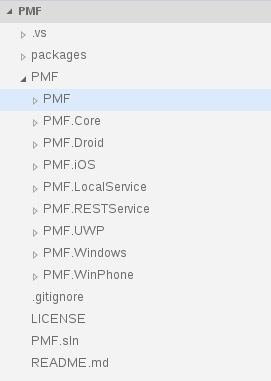
\includegraphics[width=62.92mm,height=88.46mm]{msc-img35.png}
\end{figure}
\liststyleLviii
\begin{itemize}
\item \textbf{PMF.Core} projekat predstavlja jezgro aplikacije i
kompajlira se kao portabilna biblioteka. U ovom projektu se nalaze
modeli iz domena aplikacija i svi interfejsi koji se koriste kroz
aplikaciju
\item {\bfseries
PMF.LocalService \textmd{je takođe portabilna biblioteka u kojoj se
nalaze lokalne implemetacije web servisa koje služe za testiranje
aplikacije na test podacima. U ovom projektu se nalaze servisi za
vesti, studijske programe, predmete i drugi a implementirani su pomoću
asinhronih operacija koje mogu da simuliraju zastoje na mreži i gubitak
mreže u potpunosti.}}
\item {\bfseries
PMF.RESTService \textmd{je takođe implementacija interfejsa servisa za
pristup podataka koji koristi prave RESTful web servise za pristup bazi
podataka.}}
\item {\bfseries
PMF.Droid, PMF.iOS, PMF.UWP, PMF.WinPhone, PMF.Windows \textmd{su
specifični projekti za različite platforme. U ovim projektima se nalaze
aplikacije koje se kompajliraju za različite platforme. Uglavnom sadrže
resurse koji moraju biti specifično napravljeni za specifične platforme
(npr. Slike) i samo jednu glavnu klasu aplikacije koja učitava glavnu
portabilnu biblioteku:}}
\item {\bfseries
PMF –\textmd{ glavna bilbioteka aplikacije u kojoj se nalazi sva
poslovna logika i logika korisničkog interfejsa koju dele sve
aplikacije za različite platforme.}}
\end{itemize}
\subsection[7.3. MVVM patern[13{]}]{\rmfamily 7.3. MVVM
patern\textsuperscript{[13]}}
\hypertarget{RefHeadingToc4291813786090}{}Za implementaciju glavne PMF
biblioteke koju koriste sve druge platforme korišćen je MVVM patern.



\begin{figure}
\centering
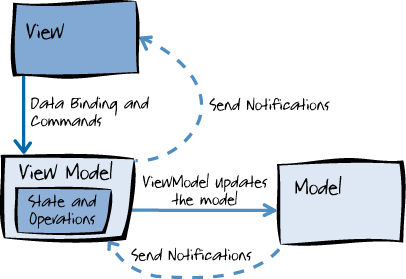
\includegraphics[width=107.42mm,height=73.82mm]{msc-img36.png}
\end{figure}
MVVM patern je veoma sličan MVC paternu sa glavnom razlikom da uvodi
koncep Data Binding-a. MVVM aplikacije pružaju dobru podelu između
različitih slojeva aplikacije i drže se principa da jedan deo
aplikacije treba da radi samo jednu stvar i da je radi nezavisno od
drugih delova. MVVM aplikacije se sastoje od tri dela:

\liststyleLix
\begin{itemize}
\item Model – sve klase domena
\item View – klase korisničkog interfejsa, često pisane u markup jeziku
(uglavnom XAML) koji podržava sintaksu za lak Data Binding
\item ViewModel – klase koje služe za povezivanje Model i View klasa.
Česta implementacija je da jedna View klasa ima tačno jednu ViewModel
klasu i prikazuje podatke koje ta ViewModel klasa sadrži. ViewModel
klase takođe sadrže detalje kao što su navigacija između drugih View
klasa i slično. ViewModel klase podatke čuvaju u C\# property-ima koji
imaju mogućnost da obaveste View klasu ukoliko dođe do izmene njihove
vrednosti kao i da automatski obrade promene vrednosti na View klasi.
Ovo se postiže implementacijom .NET INotifyPropertyChanged interfejsa.
\end{itemize}
Za primenu MVVM paterna uglavnom se koristi već postojeća biblioteka. Za
ovaj projekat odabrana je MVVMLight biblioteka zbog jednostavnosti
upotrebe i kompatibilnosti sa Xamarin projektima. Takođe, biblioteka je
besplatna i open-source. U skladu sa MVVM paternom, struktura projekta
glavne PMF biblioteke je sledeća:



\begin{figure}
\centering
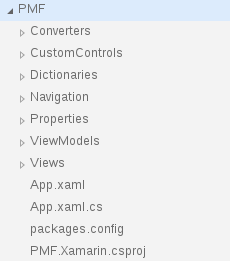
\includegraphics[width=53.2mm,height=60.36mm]{msc-img37.png}
\end{figure}

\bigskip


\bigskip

Očigledno, ne postoji deo sa domenskim klasama pošto se one koriste iz
PMF.Core biblioteke. Svi elementi korisničkog interfejsa se nalaze u
Views paketu (namespace) i svi su implementirani u XAML markup jeziku
koji će detaljniji biti opisan kasnije.

Za razmenu podataka između View i ViewModel klasa koristi se Data
Binding. Data Binding je koncept vezivanja elemenata korisničkog
interfejsa direktno sa property-ima C\# klase. Na primer u delu
aplikacije sa često postavljenim pitanjima i odgovorima u ViewModel
klasi postoji kolekcija objekata koji sadrže pitanja i odgovore i koja
se zove FAQ:



\begin{figure}
\centering
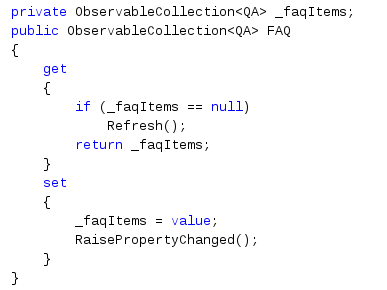
\includegraphics[width=93.56mm,height=70.1mm]{msc-img38.png}
\end{figure}
Ovaj property koristi XAML klasa
\texttt{\textcolor[rgb]{0.0,0.4,0.8}{FAQPage.xaml}} kako bi prikazala
ove objekte (samo deo prikazan): 



\begin{figure}
\centering
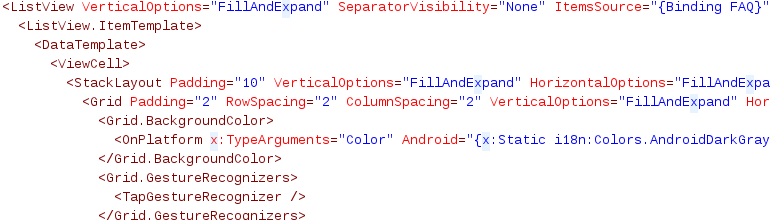
\includegraphics[width=170mm,height=48.56mm]{msc-img39.png}
\end{figure}
Važno je napomenuti da se na ovakav način ne mešaju detalji
implementacije korisničkog interfejsa (koji se nalaze u XAML kodu) i
same logike aplikacije koja se nalazi u ViewModel klasi.

Prednosti korišćenja MVVM paterna u dizajnu aplikacija sa bogatim
korisničkim interfejsom su mnoge:

\liststyleLx
\begin{itemize}
\item lakše odvojeno testiranje komonenti – testiranje XAML stranica bez
pravih podataka kao i testiranje ViewModel klasa bez korisničkog
interfejsa
\item potpuno odvajanje zaduženja klasa
\item lak redizajn interfejsa za različite platforme, ukoliko je
potrebno
\item lakše održavanje aplikacije zbog dobro struktuiranog koda
\item mogućnost podele programerskih timova na front-end i back-end
razvoj
\end{itemize}
ali postoje i mane:

\liststyleLxi
\begin{itemize}
\item neisplativo za male aplikacije, pošto se piše dosta dodatnog koda
\item sporiji razvoj
\end{itemize}
Ipak, za ozbiljnije i kompleksnije aplikacije, MVVM je standardni
pristup struktuiranju i razvoju aplikacija.

Takođe, neke delove aplikacije bi bilo nemoguće implementirati pomoću
XAML i Data Binding mogućnosti jer Xamarin biblioteka ne predviđa da
neke komponente budu korišćene na takav način. Zbog toga je bilo
potrebno implementirati dodatne komponente koje se zasnivaju na Xamarin
komponentama – biće prikazana jedna ovakva komponenta.

\subsection[7.4. Inversion of Control (IoC)[14{]}]{\rmfamily 7.4.
Inversion of Control (IoC)\textsuperscript{[14]}}
\hypertarget{RefHeadingToc852882405265}{}Kada se implementira
cross-platform nativna mobilna aplikacija, veoma je važno da komponente
budu slabo povezane i što apstraktnije. Zbog ovoga je veoma
interesantan pristup inverzije kontrole (Inversion of Control) i
Dependency Injection dizajn patern.

Koncept je veoma jednostavan. Umesto da imamo objekte koji kreiraju
druge objekte i njihove zavisne objekte, dizajniramo klase tako da ne
zavise od mesta na kojem su napravljene i same definišu svoje potrebe.
Na ovaj način se kontrola kreiranja objekata premešta iz nadobjekata
koji su tradicionalno pravili sve objekte aplikacije u same objekte
koji se instanciraju. Ovo omogućava čistiji dizajn i mnogo uredniju
strukturu samog koda.

Implementacija Dependency Injection dizajn paterna koji je samo jedan od
načina za postizanje inverzije kontrole je takođe veoma jednostavna,
sve klase po ovom dizajn paternu koriste isključivo interfejse za vezu
sa drugim objektima koji se lako mogu zameniti po potrebi.

Za implementaciju Dependency Injection dizajn paterna uglavnom se
koristi spoljašnja biblioteka. U ovoj aplikaciji korišćena je SimpleIoc
biblioteka kao deo MVVMLight biblioteke.

Ovde je prikazan deo implementacije koji koristi ovu biblioteku.



\begin{figure}
\centering
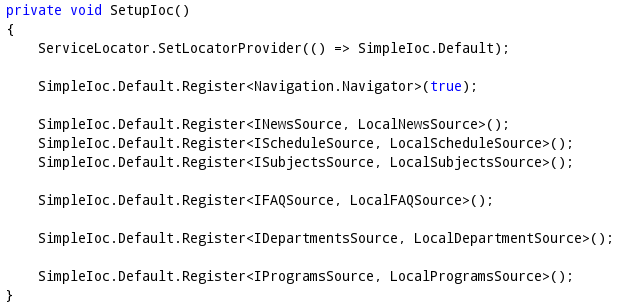
\includegraphics[width=124.97mm,height=60.03mm]{msc-img40.png}
\end{figure}
U metodu \texttt{\textcolor[rgb]{0.0,0.4,0.8}{SetupIoc}} se povezuju
interfejsi sa konkretnim implementacijama. Ovo znači da kada bilo koja
klasa u aplikaciji zatraži, npr.
\texttt{\textcolor[rgb]{0.0,0.4,0.8}{IFAQSource}} implementaciju,
dobiće instancu \texttt{\textcolor[rgb]{0.0,0.4,0.8}{LocalFAQSource}}
klase.

Na primer, u konstruktoru
\texttt{\textcolor[rgb]{0.0,0.4,0.8}{FAQViewModel}} klase nam je
potrebna instanca servisa za česta pitanja i odgovore i tu koristimo
IoC kontejner da dobijemo konkretnu implementaciju. Na ovaj način
nikada sami ne kreiramo objekte, već puštamo kontejner da to uradi za
nas i da se stara da uvek dobijamo objekat koji želimo da dobijemo.
Zbog jednostavnosti upotrebe SimpleIoc biblioteka i generalno koncept
inverzije kontrole je veoma koristan za kreiranje singleton objekata
(singleton objekat je objekat koji uvek ima samo jednu instancu), te se
u ovoj aplikaciji koristi i za kreiranje ViewModel klasa (samo deo
prikazan):

\begin{figure}
\centering
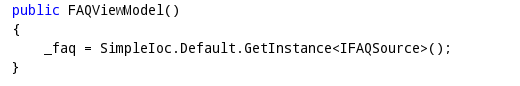
\includegraphics[width=128.85mm,height=21.31mm]{msc-img41.png}
\end{figure}
 

\begin{figure}
\centering
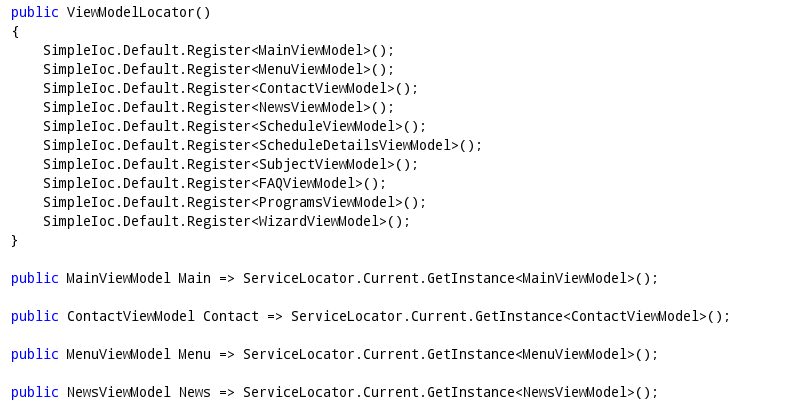
\includegraphics[width=170mm,height=55.65mm]{msc-img42.png}
\end{figure}
a takođe i za \texttt{\textcolor[rgb]{0.0,0.4,0.8}{ViewLocator}} klasu
koja služi za lociranje View objekata:



\begin{figure}
\centering
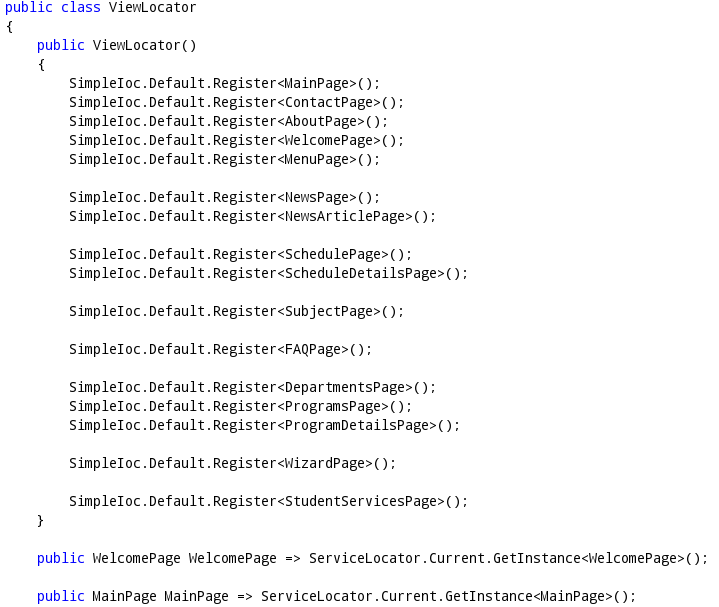
\includegraphics[width=150.67mm,height=69.39mm]{msc-img43.png}
\end{figure}
Ovo u mnogome olakšava rad sa kompleksnim View i ViewModel klasama kojih
ima mnogo. Takođe, klase
\texttt{\textcolor[rgb]{0.0,0.4,0.8}{ViewModelLocator}} i
\texttt{\textcolor[rgb]{0.0,0.4,0.8}{ViewLocator}} su napisane na takav
način da se mogu koristiti direktno bilo gde iz koda čak i iz XAML
fajlova.

\subsection[7.5. Resursi aplikacije]{\rmfamily 7.5. Resursi aplikacije}
\hypertarget{RefHeadingToc854882405265}{}Kada se razvija ovakav tip
aplikacije, česta je potreba da se definišu globalni resursi
aplikacije. Ovo mogu biti razni pomoćni objekti koji se koriste kroz
celu aplikaciju. Koncept inverzije kontrole prikazan u prošlom
poglavlju nam donekle može pomoći, međutim ostaje problem lociranja
samih „lokator“ klasa koje se negde moraju definisati. 

Po konvenciji (generalno u .NET aplikacijama koje koriste XAML) ovo je
\texttt{\textcolor[rgb]{0.0,0.4,0.8}{App.xaml}} fajl.

\texttt{\textcolor[rgb]{0.0,0.4,0.8}{App.xaml}} fajl i propratna
\texttt{\textcolor[rgb]{0.0,0.4,0.8}{App.xaml.cs}} klasa su glavna
ulazna tačka aplikacije i mogu sadržati definiciju resursa aplikacije.
Pri kompajliranju \texttt{\textcolor[rgb]{0.0,0.4,0.8}{App.xaml}}
klase, klase koje su navedene kao resursi biće instancirane sa
podrazumevanim konstruktorima i smeštene u memoriju. Odatle će im biti
veoma lako pristupiti bilo gde iz aplikacije, bilo iz C\# klasa ili
XAML klasa.

Sadržaj \texttt{\textcolor[rgb]{0.0,0.4,0.8}{App.xaml}} fajla:



\begin{figure}
\centering
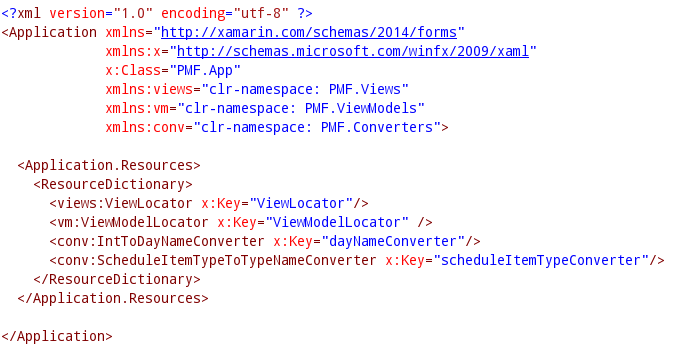
\includegraphics[width=170mm,height=85mm]{msc-img44.png}
\end{figure}
Resursi se definišu u
\texttt{\textcolor[rgb]{0.0,0.4,0.8}{Application.Resources}}
promenljivi koristeći se posebnim rečnikom sa parovima ključ i
vrednost. Naravno ovde se navode samo željeni ključevi, dok će
vrednosti biti instance objekata. Ovim instancama objekata kasnije se
pristupa na veoma jednostavan način:



\begin{figure}
\centering

\includegraphics[width=170mm,height=4.41mm]{msc-img45.png}
\end{figure}
ili iz XAML koda:

sa ključnom reči \texttt{\textcolor[rgb]{0.0,0.4,0.8}{StaticResource}} i
navedenim ključem.

\begin{figure}
\centering
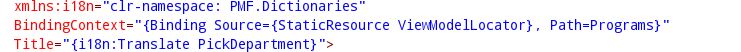
\includegraphics[width=170mm,height=11.92mm]{msc-img46.png}
\end{figure}
\subsection[7.6. Navigacija ]{\rmfamily 7.6. Navigacija }
\hypertarget{RefHeadingToc856882405265}{}Kada se razvijaju MVVM
aplikacije, bilo mobilne ili desktop, veoma velik problem je navigacija
između raznih ekranskih formi. Problem je što po principima MVVM
paterna, View klase ne bi trebalo da znaju ništa o postojanju drugih
View klasa a ni o ViewModel klasi za koju su vezane. Takođe, česta je
diskusija o tome gde bi trebalo smestiti deo koda koji će raditi
navigaciju da li u ViewModel klasu ili u View klasu. Implementacija
zavisi od programera do programera, često se pojavljuju rešenja gde će
cela aplikacija biti implementirana po MVVM principu bez navigacije,
koja će biti naknadno dodata kao klasičan event-driven deo aplikacije.
Autor ovog rada se odlučio da ne odustane od MVVM principa u ovom
slučaju i da implementira (po njegovom mišljenju) dobar način
navigacije kroz aplikaciju.

Važno je napomenuti da je aplikacija za studentske servise Master-Detail
aplikacija. To znači da postoje dve centralne komponente aplikacije
Master strana, koja se nikada ne menja (u ovom slučaju to je meni
aplikacije) i Detail strana koja prikazuje sadržaj. Implementacija se
lako vidi u fajlu \texttt{\textcolor[rgb]{0.0,0.4,0.8}{MainPage.xaml}}:

Ova implementacija se oslanja na
\texttt{\textcolor[rgb]{0.0,0.4,0.8}{MasterDetailPage}} klasu iz
Xamarin.Forms biblioteke.

\begin{figure}
\centering
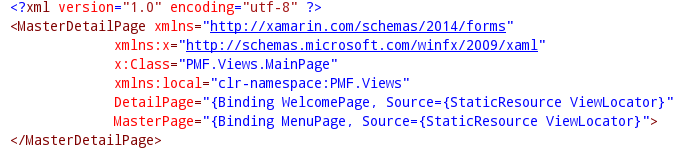
\includegraphics[width=140.72mm,height=31.63mm]{msc-img47.png}
\end{figure}
Donekle, ovo olakšava navigaciju. Ukoliko imamo referencu na glavnu
stranu (koju lako možemo dobiti pomoću
\texttt{\textcolor[rgb]{0.0,0.4,0.8}{ViewLocator}} klase) možemo da
pristupimo \texttt{\textcolor[rgb]{0.0,0.4,0.8}{DetailPage}} polju i da
ga promenimo instancom željene strane – koju takođe možemo dobiti iz
\texttt{\textcolor[rgb]{0.0,0.4,0.8}{ViewLocator}} klase.
Implementirana je odvojena klasa
\texttt{\textcolor[rgb]{0.0,0.4,0.8}{Navigator}} čija jedina svrha je
da navigira između stranica aplikacije. Na primer, kod za navigaciju sa
jedne stranice na drugu:

Kao parametar se šalje tip tj. klasa stranice koju želimo da prikažemo
korisniku. Ovo je pogotovo korisno jer ne ostavljamo mesta za greške, u
poređenju da se na primer ime strane prosledi kao string. Takođe,
SimpleIoc biblioteka ima metod koji za prosleđeni tip klase vraća njenu
implementaciju, što dovodi do veoma jednostavne implementacije.

\begin{figure}
\centering
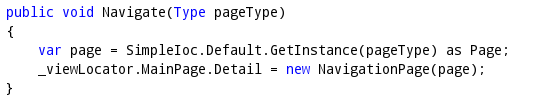
\includegraphics[width=112.18mm,height=22.1mm]{msc-img48.png}
\end{figure}
Kada neka stranica želi da navigira na drugu stranicu, tj. kada korisnik
naznači da želi da ode na neku drugu stranicu na primer klikom na
dugme, tada stranica kroz komandu na svom ViewModel-u javlja
\texttt{\textcolor[rgb]{0.0,0.4,0.8}{Navigator}} klasi da uradi
navigaciju. Na primer za otvaranje detalja predmeta u aplikaciji:



\begin{figure}
\centering
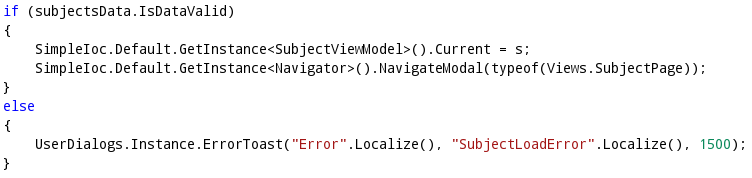
\includegraphics[width=170mm,height=40.23mm]{msc-img49.png}
\end{figure}
Pre samog poziva za navigaciju, potrebno je i osvežiti odgovarajuću
ViewModel klasu kako bi podaci bili ažurni.

\subsection[7.7. Lokalizacija]{\rmfamily 7.7. Lokalizacija}
\hypertarget{RefHeadingToc858882405265}{}Aplikacija za studentske
servise je lokalizovana na više jezika: srpski (ćirilica i latinica),
engleski, i mađarski. Ovo se postiže ne korišćenjem eksplicitno
definisanih string-ova (hard-coded strings) u korisničkom interfejsu
već korišćenjem rečnika pojmova za svaki jezik pojedinačno.

Xamarin biblioteka podržava lokalizaciju aplikacija. Koriste se
standardni .NET rečnici resursa (.resx) fajlovi koji se zatim
kompajliraju u C\# klase sa konstantama. Na primer, deo rečnika za
engleski jezik u ResX formatu:

\begin{figure}
\centering
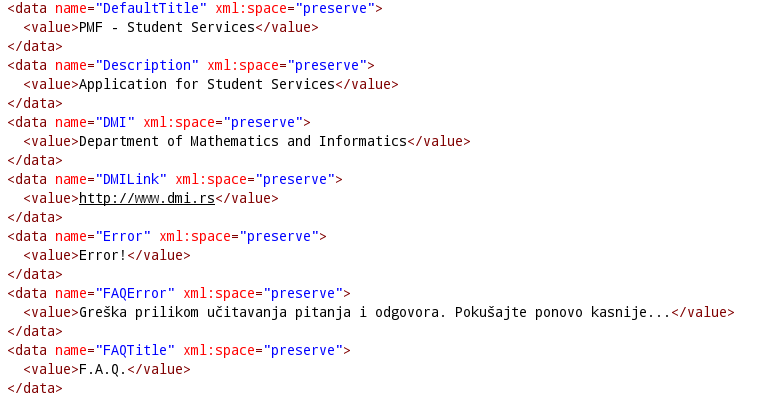
\includegraphics[width=154.78mm,height=79.67mm]{msc-img50.png}
\end{figure}
i odgovarajuća C\# klasa:



\begin{figure}
\centering
\includegraphics[width=138.09mm,height=68.53mm]{msc-img51.png}
\end{figure}
ResX rečnici se mogu definisati u samom XML-u ili kroz vizuelni alat
koji se nalazi u razvojnom okruženju. Za ključeve se korišćeni termini
na engleskom jeziku pošto se oni zapravo koriste u kodu aplikacije koji
je na engleskom jeziku.

Nažalost, osim podrške za kompajliranje ResX rečnika, Xamarin biblioteka
nam ne pruža mnogo naprednih mogućnosti za korišćenje istih, te su zbog
toga morale biti implementirane dodatne pomoćne klase. Pri
implementaciji ovih dodatnih klasa vodilo se računa da budu kratke,
brze, i da se mogu ponovo koristiti u budućim projektima.

Autor ovog teksta se ovde odlučio za upotrebu jedne od moćnijih
mogućnosti C\# programskog jezika – ekstenzione metode. Ekstenzioni
metodi (Extension Method) su metodi koji se mogu „prilepiti“ na klasu
bez da se ona nasledi i ponovo instancira. Prirodno je bilo napraviti
ovakav metod za string klasu koji može da lokalizuje bilo koji ključ, i
koji za na koji jezik treba da ga prevede:

Dakle, sve što je potrebno da bi se lokalizovala vrednost je da se
pozove \texttt{\textcolor[rgb]{0.0,0.4,0.8}{Localize}} metod nad nekom
string promenljivom. Na primer:

\begin{figure}
\centering
\includegraphics[width=115.85mm,height=69mm]{msc-img52.png}
\end{figure}
Ovaj metod se može pozvati i na samoj definiciji string-a, kao što je
ovde i prikazano. 

\begin{figure}
\centering
\includegraphics[width=170mm,height=18.43mm]{msc-img53.png}
\end{figure}
\texttt{\textcolor[rgb]{0.0,0.4,0.8}{Translator}} klasa se stara da
lokalizacija bude na predviđenom jeziku, i da program nastavi svoje
izvršavanje čak i ako ne postoji prevedena vrednost ključa.

Naravno, većina elemenata koje je bilo potrebno prevoditi na razne
jezike se nije nalazio u C\# kodu već u XAML kodu gde je i definisan
korisnički interfejs.

Za korišćenje Translator klase iz XAML koda bilo je takođe potrebno
implementirati i ekstenziju samog XAML jezika za markiranje. Naravno,
moguća je i jednostavnija implementacija, ali ovakav način je ispravan
sa aspekta čistoće koda i daleko najfleksibilnija opcija. 

Ekstenzije se u XAML kodu definišu implementacijom specijalnog
interfejsa \texttt{\textcolor[rgb]{0.0,0.4,0.8}{IMarkupExtension}}:

Takođe je potrebno naglasiti da ova ekstenzija radi sa vrednostima, a ne
sa samim delovima XAML koda. Kada je ovakva ekstenzija napravljena,
veoma je lako koristiti naš
\texttt{\textcolor[rgb]{0.0,0.4,0.8}{Translator.Localize}} metod bilo
gde iz XAML koda. Prvo se mora definisati upotreba same ekstenzije, a
za to je dovoljno samo da kažemo u kojem se paketu (namespace) nalazi.
Ovo se najčešće radi u prvom elementu stranice, jer onda svi
podelementi nasleđuju tu definiciju:

\begin{figure}
\centering
\includegraphics[width=110.95mm,height=38.96mm]{msc-img54.png}
\end{figure}
{\itshape
Napomena: svuda je korišćeno ime „i18n“ kao univerzalna programerska
oznaka za internacionalizaciju koda tj. lokalizaciju (18 je broj slova
u engleskoj reči internationalization između prvog „i“ i poslednjeg
„n“)}

\begin{figure}
\centering
\includegraphics[width=170mm,height=30.43mm]{msc-img55.png}
\end{figure}
Zatim se ekstenzija može koristiti bilo gde u kodu korišćenjem
\texttt{\textcolor[rgb]{0.0,0.4,0.8}{i18n:Translate}} direktive:

\begin{figure}
\centering
\includegraphics[width=127.48mm,height=52.95mm]{msc-img56.png}
\end{figure}
\subsection[7.8. Ekstenzije XAML komponenti]{\rmfamily 7.8. Ekstenzije
XAML komponenti}
\hypertarget{RefHeadingToc860882405265}{}Pored ove ekstenzije za
lokalizaciju, u razvoju aplikacije bilo je potrebno implementirati
dodatne XAML komponente koje se oslanjaju na Xamarin-ove
implementacije.

Razlog za ovo je što je Xamarin.Forms biblioteka još uvek u razvoju i
neke funkcionalnosti nisu moguće ukoliko se koristi XAML kod za
definiciju interfejsa. U ovakvim slučajevima postoje samo dva rešenja:
implementacija celog korisničkog interfejsa u C\# kodu, ili definicija
dodatnih komponenti. 

Ovakvi problemi se uglavnom odnose na nemogućnost korišćenja Data
Binding-a (pa ni MVVM paterna) na neke promenljive već postojećih
komponenti, što veoma narušava strukturu i dizajn koda aplikacije.

\subsubsection[]{\rmfamily }
\clearpage\subsubsection[7.8.1. Implementacija PinMap
komponente]{\rmfamily 7.8.1. Implementacija PinMap komponente}
\hypertarget{RefHeadingToc862882405265}{}U Xamarin biblioteci postoji
\texttt{\textcolor[rgb]{0.0,0.4,0.8}{Map}} komponenta koja predstavlja
geografsku mapu. Velika prednost ove komponente je što radi na svim
mobilnim uređajima nezavisno od platforme, tj. povezuje se na
odgovrajućeg provider-a navigacionih usluga: Google Maps za Android,
Apple Maps za iOS, Bing Maps za Windows.

Ova komponenta je jedna od najrazvijanijih komponenti Xamarin.Forms
biblioteke, ali i pored toga ne postoji mogućnost postavljanja
takozvanog Pin-a (grafičkog obeležja lokacije na mapi) kroz XAML kod.
Zbog toga, ovde je implementirana komponenta
\texttt{\textcolor[rgb]{0.0,0.4,0.8}{PinMap}} koja se oslanja na
komponentu \texttt{\textcolor[rgb]{0.0,0.4,0.8}{Map}} iz Xamarin.Forms
biblioteke ali ima mogućnost definisanja geografske širine i dužine na
kojoj će biti postavljen Pin odmah pri konstrukciji objekta. Takođe, po
postavljanju Pin-a \texttt{\textcolor[rgb]{0.0,0.4,0.8}{PinMap}}{}-a će
automatski prikazati lokaciju tog Pin-a tačno na sredini mape uz
odgovarajuću animaciju – što takođe nije moguće iz XAML koda sa običnom
Map komponentom.

\begin{figure}
\centering
\includegraphics[width=170mm,height=98.09mm]{msc-img57.png}
\end{figure}
Takođe, moguće je definisati i šta će pisati na samom Pin-u i sa koje
udaljenosti (u metrima) će biti prikazan. U setter-u polja
\texttt{\textcolor[rgb]{0.0,0.4,0.8}{NavigateImmediately}} se nalazi
poziv funkciji \texttt{\textcolor[rgb]{0.0,0.4,0.8}{NavigateNow}} koja
će postaviti Pin na mapu i prikazati ga sa određene udaljenosti. Ovo je
veoma jednostavan način za pozivanje metoda direktno iz XAML koda –
svaka promena vrednosti će okinuti setter prekidač koji će tada pozvati
navedeni metod.

Ovako napravljene XAML komponente koriste se slično kao i ekstenzije
koje su bile prikazane u prošlom poglavlju. Prvo se definiše u kom su
paketu (maps):

A zatim se normalno koriste sa prefiksom:

\begin{figure}
\centering
\includegraphics[width=170mm,height=18.77mm]{msc-img58.png}
\end{figure}


\begin{figure}
\centering
\includegraphics[width=170mm,height=41.52mm]{msc-img59.png}
\end{figure}
U ovakvoj definiciji, polja
\texttt{\textcolor[rgb]{0.0,0.4,0.8}{Latitude}},
\texttt{\textcolor[rgb]{0.0,0.4,0.8}{Longitude}},
\texttt{\textcolor[rgb]{0.0,0.4,0.8}{PinTitle}},
\texttt{\textcolor[rgb]{0.0,0.4,0.8}{PinDistance}},
\texttt{\textcolor[rgb]{0.0,0.4,0.8}{NavigateImmediately}} su sva iz
PinMap klase koja je naknadno definisana. Na ovaj način ne gubimo na
urednosti koda, a ni na kompatibilnosti sa različitim platformama,
pošto je ovo i dalje u osnovi Xamarin.Forms komponenta koja može da se
koristi na svim platformama. 

Ovde je prikazana komponenta na iOS platformi:

\subsubsection[]{\rmfamily }
\begin{figure}
\centering
\includegraphics[width=64.49mm,height=114.72mm]{msc-img60.png}
\end{figure}
\clearpage\subsubsection[7.8.2. Implementacija ExtendedPicker
komponente]{\rmfamily 7.8.2. Implementacija ExtendedPicker komponente}
\hypertarget{RefHeadingToc864882405265}{}Još jedna komponenta koja je
nedostajala je \texttt{\textcolor[rgb]{0.0,0.4,0.8}{Picker}} (slično
\texttt{\textcolor[rgb]{0.0,0.4,0.8}{ComboBox}} komponenti u drugim
bibliotekama) koja ima mogućnost Data Binding-a.

Većina kompozitnih komponenti iz Xamarin.Forms biblioteke kao što su
\texttt{\textcolor[rgb]{0.0,0.4,0.8}{ListView}} ili
\texttt{\textcolor[rgb]{0.0,0.4,0.8}{TableView}} definišu polje
\texttt{\textcolor[rgb]{0.0,0.4,0.8}{ItemsSource}} koje se može
manipulisati uz pomoć DataBinding-a. Međutim, iz nekog razloga ovo nije
slučaj sa \texttt{\textcolor[rgb]{0.0,0.4,0.8}{Picker}} komponentom, te
je bila potrebna dodatna implementacija.



\begin{figure}
\centering
\includegraphics[width=170mm,height=81.93mm]{msc-img61.png}
\end{figure}
Implementacija je malo komplikovanija od implementacije
\texttt{\textcolor[rgb]{0.0,0.4,0.8}{PinMap}} komponente zbog
neophodnosti da se koristi koncept
\texttt{\textcolor[rgb]{0.0,0.4,0.8}{BindableProperty}}. Kao što mu ime
kaže \texttt{\textcolor[rgb]{0.0,0.4,0.8}{BindableProperty}} je polje
klase koje podržava Data Binding. Ovakav kod uglavnom ne piše programer
već se on sam generiše, međutim u ovom slučaju ovo je bilo jedino
rešenje. Dakle, postoji obična lista
\texttt{\textcolor[rgb]{0.0,0.4,0.8}{string}} objekata koje želimo da
povežemo sa \texttt{\textcolor[rgb]{0.0,0.4,0.8}{Picker}} objektom.
Definičemo \texttt{\textcolor[rgb]{0.0,0.4,0.8}{BindableProperty}} uz
pomoć .NET metoda
\texttt{\textcolor[rgb]{0.0,0.4,0.8}{BindableProperty.Create}} i dajemo
mu ime, tip, i u specijalnom lambda izrazu definišemo šta se dešava
kada se vrednost ove promeljive promeni – u našem slučaju jednostavno u
instanci same \texttt{\textcolor[rgb]{0.0,0.4,0.8}{Picker}} komponente
očistimo postojeću listu i dodamo sve elemente nove liste. 

Ovakav kod je generički, i nije podležan promenama a u mnogome olakšava
dalji rad sa \texttt{\textcolor[rgb]{0.0,0.4,0.8}{Picker}} komponentom
kada nam je potrebna mogućnost Data Binding-a na kolekciju objekata
koju prikazuje:



\begin{figure}
\centering
\includegraphics[width=170mm,height=33.13mm]{msc-img62.png}
\end{figure}
Ovakve mogućnosti „dodavanja“ komponenti na samu biblioteku uz pomoć
naprednih koncepata koje pruža programski jezik C\# umnogome olakšavaju
razvoj ovakvog tipa aplikacija.

\subsubsection[7.8.3. XAML konverteri]{\rmfamily 7.8.3. XAML konverteri}
\hypertarget{RefHeadingToc866882405265}{}Prilikom lokalizacije
aplikacije, došlo je do problema lokalizacije vrednosti tipa
\texttt{\textcolor[rgb]{0.0,0.4,0.8}{enum}}. Pošto se ovakvi tipovi
podataka u C\# programskom jeziku mapiraju na vrednosti tipa
\texttt{\textcolor[rgb]{0.0,0.4,0.8}{int}}, nije postojao jednostavan
način za lokalizaciju samih imena
\texttt{\textcolor[rgb]{0.0,0.4,0.8}{enum}} vrednosti. Zbog ovoga,
korišćeni su XAML konverteri.

XAML konverter je jednostavna klasa koja implementira interfejs
\texttt{\textcolor[rgb]{0.0,0.4,0.8}{IValueConverter}} i implementira
dva njegova metoda: \texttt{\textcolor[rgb]{0.0,0.4,0.8}{Convert}} i
\texttt{\textcolor[rgb]{0.0,0.4,0.8}{ConvertBack}}. Na primer, XAML
konverter koji lokalizuje tipove predavanja (predavanje, vežbe ili
vežbe na računaru):

U ovom slučaju nam nije potrebna implementacija prevođenja unazad, te
taj metod nije ni implementiran. Lokalizovane vrednosti se čuvaju u
rečniku (ključ-vrednost parovi) a sam XAML kod poziva
\texttt{\textcolor[rgb]{0.0,0.4,0.8}{Convert}} metod za nas:

\begin{figure}
\centering
\includegraphics[width=170mm,height=79.15mm]{msc-img63.png}
\end{figure}


\begin{figure}
\centering
\includegraphics[width=170mm,height=31.59mm]{msc-img64.png}
\end{figure}
XAML konverteri su definisani i instancirani u
\texttt{\textcolor[rgb]{0.0,0.4,0.8}{App.xaml}} klasi. 

Još jedan interesantan konverter je za dane u nedelji i njihova
lokalizovana imena:



\begin{figure}
\centering
\includegraphics[width=170mm,height=96.36mm]{msc-img65.png}
\end{figure}
XAML konverteri su moćno oruđe za konverziju podataka koji nam ponovo
pomažu da što više koda generalizujemo i izmestimo van korisničkog
interfejsa.

\subsection[7.9. Kod za specifične platfome]{\rmfamily 7.9. Kod za
specifične platfome}
\hypertarget{RefHeadingToc873882405265}{}Iako je većina koda u PCL
projektu nezavisna od platforme na kojoj se izvršava, Xamarin
biblioteka nam pruža neke mogućnosti za provere na kojoj se platformi
aplikacija trenutno izvršava, ukoliko nam je takva informacija
potrebna. Ovo je veoma korisno u dizajno korisničkog interfejsa,
ukoliko želimo da izgleda nešto drugačije na različitim platformama
kako bi se uklopio u ostatak izgleda operativnog sistema. Na primer u
XAML kodu možemo da definišemo različite boje komponenti na različitim
platformama ili čak različite numeričke vrednosti za razne osobine – u
ovom primeru visinu komponente:



\begin{figure}
\centering
\includegraphics[width=170mm,height=36.78mm]{msc-img66.png}
\end{figure}
Kod koji će se izvršavati samo na određenim platformama moguće je pisati
i u samim C\# klasama na sledeći način:

U ovom primeru za iOS platformu je potrebna drugačija implementacija
prikaza poruke, jer ta platforma ne podržava dijaloge koji imaju više
od jednog reda.

\begin{figure}
\centering
\includegraphics[width=170mm,height=109.26mm]{msc-img67.png}
\end{figure}
Iako se ovakve konstrukcije retko koriste, u većini slučajeva kada su
potrebne, zapravo su nezamenljive i neki delovi koda se moraju
implementirati na ovaj način.

\subsection[7.10. Pristup naprednijim mogućnostima mobilnih uređaja na
jedinstven način]{\rmfamily 7.10. Pristup naprednijim mogućnostima
mobilnih uređaja na jedinstven način}
\hypertarget{RefHeadingToc875882405265}{}Iako je Xamarin biblioteka u
potpunosti cross-platform, u nekim slučajevima mora se pisati kod
specifičan za platformu na kojoj se aplikacija izvršava, kao što smo
videli u prethodnom poglavlju.

Napredne mogućnosti mobilnih uređaja kao što su kamera, notifikacije,
pozivi i poruke i slično se veoma razlikuju od platforme do platforme i
još ne postoji jedinstveni način za pristup istima.

Trenutno postoji mnogo open-source biblioteka koje rade upravo ovo, i
zbog njih ne moramo da pišemo kod za specifične platforme, jer se takav
kod već nalazi u njima. U razvoju aplikacije za studentske servise
korišćene su mnoge ovakve biblioteke.

Važno je napomenuti da je korišćenje ovakvih biblioteka moguće samo u
projektima koji koriste PCL biblioteku kao osnovu ali ne i u takozvanim
Shared projektima, te je ovo još jedan od razloga zbog kojih je bolje
krenuti u razvoj uz pomoć PCL biblioteke.

\subsubsection[7.10.1. Notifikacije]{\rmfamily 7.10.1. Notifikacije}
\hypertarget{RefHeadingToc877882405265}{}Na žalost nije moguće na
jedinstven način kontrolisati notifikacije tj. Kratke poruke prikazane
korisniku na svim različitim platformama.

Zbog ovoga je korišćena odlična open-source biblioteka
\texttt{\textcolor[rgb]{0.0,0.4,0.8}{Acr.UserDialogs}}\textsuperscript{[15]}.
Ova biblioteka je veoma jednostavna za korišćenje, koristi se jedan
singleton objekat:

Poziv funkcije prima tri parametra: sadržaj, naslov i dužinu trajanja
poruke u milisekundama. Takođe osim ovde prikazane
\texttt{\textcolor[rgb]{0.0,0.4,0.8}{Error}} poruke, postoje i druge
razne kao što su \texttt{\textcolor[rgb]{0.0,0.4,0.8}{Success}} ili
\texttt{\textcolor[rgb]{0.0,0.4,0.8}{Info}} poruke koje se razlikuju po
izgledu.

\begin{figure}
\centering
\includegraphics[width=170mm,height=5.59mm]{msc-img68.png}
\end{figure}
\subsubsection[]{\rmfamily }
\clearpage\subsubsection[7.10.2. Poruke i dijalozi]{\rmfamily 7.10.2.
Poruke i dijalozi}
\hypertarget{RefHeadingToc879882405265}{}Za prikaz drugih,
komplikovanijih poruka i dijaloga može se koristiti ista biblioteka.
Dijalozi se prave takođe na jednostavan način:

i izgledaju kao nativni dijalozi na svim platformama, na primer iOS i
Android:

\begin{figure}
\centering
\includegraphics[width=170mm,height=56.59mm]{msc-img69.png}
\end{figure}

\bigskip

\subsubsection[]{\rmfamily }
\begin{figure}
\centering
\includegraphics[width=50.09mm,height=89.09mm]{msc-img70.png}
\end{figure}
\begin{figure}
\centering
\includegraphics[width=50.17mm,height=89.25mm]{msc-img71.png}
\end{figure}
\subsubsection[7.10.3. Otvaranje linkova u podrazumevanom internet
pregledaču]{\rmfamily 7.10.3. Otvaranje linkova u podrazumevanom
internet pregledaču}
\hypertarget{RefHeadingToc881882405265}{}Još jedna od mogućnosti koja
nedostaje u Xamarin biblioteci je otvaranje jednostavnih linkova do web
stranica u podrazumevanom web pregledaču koji korisnik podešava.
Srećom, postoji open-source biblioteka koja služi samo za ovo
(\texttt{\textcolor[rgb]{0.0,0.4,0.8}{CrossShare}}):

Jedini nedostatak biblioteke je što ukoliko link ne počinje sa
standardnim \texttt{\textcolor[rgb]{0.0,0.4,0.8}{http://}} ili
\texttt{\textcolor[rgb]{0.0,0.4,0.8}{https://}} prefiksom već direktno
sa adresom (npr. \texttt{\textcolor[rgb]{0.0,0.4,0.8}{www.google.com}})
stranica se neće otvoriti, te se taj slučaj mora ručno obraditi. Nakon
pozivanja metoda \texttt{\textcolor[rgb]{0.0,0.4,0.8}{OpenBrowser}},
korisniku će biti prikazan podrazumevani web pregledač i to u okviru
naše aplikacije za studentske servise kao modalni dijalog:

\begin{figure}
\centering
\includegraphics[width=153.46mm,height=36.78mm]{msc-img72.png}
\end{figure}


\begin{figure}
\centering
\includegraphics[width=59.67mm,height=106.13mm]{msc-img73.png}
\end{figure}
Ovo je veoma važna opcija jer se korisnik lako može vratiti direktno u
aplikaciju pritiskom na odgovarajuće dugme.

\subsubsection[7.10.4. Deljenje linkova, slanje e{}-mail
poruka]{\rmfamily 7.10.4. Deljenje linkova, slanje e-mail poruka}
\hypertarget{RefHeadingToc883882405265}{}Slanje e-mail poruka preko
predefinisane aplikacije za mejlove je takođe nemoguće bez dodatne
biblioteke.

Za ovu mogućnost koristi se takođe
\texttt{\textcolor[rgb]{0.0,0.4,0.8}{CrossShare}}\textsuperscript{[16]}
biblioteka:



\begin{figure}
\centering
\includegraphics[width=170mm,height=39.88mm]{msc-img74.png}
\end{figure}
Po pozivu metoda \texttt{\textcolor[rgb]{0.0,0.4,0.8}{SendEmail}} koji
prima adresu, naslov, i sadržaj poruke kao parametre, korisniku će biti
prikazan dijalog da odabere sa koje e-mail adrese želi da pošalje
poruku (ukoliko korisnik ima više e-mail adresa podešenih) i zatim
popunjena e-mail poruka, spremna za slanje.

Još jedna važna mogućnost modernih mobilnih aplikacija je mogućnost
deljenja linkova i sadržaja na raznim društvenim mrežama. Srećom, svi
operativni sistemi koje Xamarin biblioteka podržava definišu interfejse
koji nam omogućavaju upravo ovo. Nažalost, svaki operativni sistem
definiše različit interfejs, te nam je ponovo potrebna biblioteka.
Ponovo koristimo \texttt{\textcolor[rgb]{0.0,0.4,0.8}{CrossShare}}:



\begin{figure}
\centering
\includegraphics[width=151.15mm,height=121.87mm]{msc-img75.png}
\end{figure}
Ovaj deo koda omogućava korisniku da „podeli“ ili snimi lokalno (u
aplikacijama koje to podržavaju ili u memoriju – clipboard) listu
predmeta koje je odabrao za prijavu semestra. Samo Android platforma
podržava snimanje teksta u clipboard, te je ta opcija jedino prikazana
na toj platformi. 

Kod je veoma jednostavan, koristi se
\texttt{\textcolor[rgb]{0.0,0.4,0.8}{StringBuilder}} za pravljenje
poruke koja se zatim jednostavno prosleđuje metodu
\texttt{\textcolor[rgb]{0.0,0.4,0.8}{Share}} iz
\texttt{\textcolor[rgb]{0.0,0.4,0.8}{CrossShare}} biblioteke.

\subsubsection[7.10.5. Keširanje slika]{\rmfamily 7.10.5. Keširanje
slika}
\hypertarget{RefHeadingToc885882405265}{}Pošto je cilj razvoja
cross-platform mobilne aplikacije da što više korisnika ima mogućnost
da je koristi, mora se voditi računa i o performansama. 

Kada je reč o telefonima starijih generacija ili limitiranih
performansi, veoma je korisno koristiti keširanje za velike slike koje
se koriste na više mesta kroz aplikaciju. Na primer, u prikazu
rasporeda časova koristi se velika slika ukoliko je raspored prazan:



\begin{figure}
\centering
\includegraphics[width=46.92mm,height=83.5mm]{msc-img76.png}
\end{figure}
\begin{figure}
\centering
\includegraphics[width=48.98mm,height=87.14mm]{msc-img77.png}
\end{figure}

\bigskip

koja se može ponavljati više dana u nedelji. Iako na prvi pogled u ovom
slučaju keširanje izgleda nepotrebno, bilo kakvo šteđenje RAM memorije
mobilnog uređaja je veoma korisno, i unapređuje performanse ostalih
delova aplikacije. 

Takođe, u aplikaciji za studentske servise keširaju se i slike koje se
preuzimaju preko mreže, što takođe smanjuje prenešene podatke što je
veoma važno na mobilnim uređajima.

Za keširanje slika ne postoji ugrađen mehanizam u samoj Xamarin
biblioteci, već se koristi eksterna biblioteka
\texttt{\textcolor[rgb]{0.0,0.4,0.8}{FFImageLoading}}\textsuperscript{[17]}
direktno iz XAML koda:



\begin{figure}
\centering
\includegraphics[width=170mm,height=41.01mm]{msc-img78.png}
\end{figure}
Ova bibloteka koristi ime fajla tj. URL do slike ukoliko se ona preuzima
sa mreže kao ključ za keširanje. Takođe se može podesiti u dužina
važenja slike u memoriji, animacije i slično.


\bigskip

\clearpage\section[8. Zaključak]{\rmfamily 8. Zaključak}
\hypertarget{RefHeadingToc889882405265}{}\clearpage\section[Reference]{\rmfamily
Reference}
\hypertarget{RefHeadingToc887882405265}{}[1] Albahari J., Albahari B.,
C\# 6.0 in a Nutshell (Sixth Edition), O{\textquotesingle}Reilly Media,
November 2015, 1136 p, 9781491927069 

[2] C\# i .NET MSDN dokumentacija,
\url{https://msdn.microsoft.com/library} 

[3] Hermes D., Xamarin Mobile Application Development, Apress, July
2015, 432p, ISBN: 9781484202159 

[4] Michaelis M., Lippert E., Essential C\# 6.0 (Fifth Edition),
Addison-Wesley Professional, October 2015, 1008p, ISBN: 9780134141046 

[5] Peppers J., Xamarin Cross-platform Application Development, Packt
Publishing, February 2015, 262p, ISBN: 9781849698467 

[6] Petzold C., Creating Mobile Apps with Xamarin.Forms Book Preview,
Microsoft Press, April 2015, 448p, ASIN: B00VYSSNJW 

[7] Xamarin dokumentacija, \url{https://developer.xamarin.com/api/} 

\clearpage\section[Web linkovi i druge reference (iz samog rada)]{Web
linkovi i druge reference (iz samog rada)}
\hypertarget{RefHeadingToc1454255603686}{}[1]
\url{https://cordova.apache.org/} 

[2] \url{https://www.nativescript.org/} 

[3] \url{https://facebook.github.io/react-native/} 

[4]
\url{https://code.facebook.com/posts/895897210527114/dive-into-react-native-performance/}

[5] \url{https://www.codenameone.com/} 

[6] \url{https://kivy.org/#home} 

[7] \url{https://www.xamarin.com/} 

[8] \url{http://www.mono-project.com/} 

[9] \url{https://www.xamarin.com/forms} 

[10] \url{https://msdn.microsoft.com/en-us/library/cc295302.aspx} 

[11] \url{http://jeffreypalermo.com/blog/the-onion-architecture-part-1/}


[12]
\url{https://msdn.microsoft.com/en-us/library/gg597391(v=vs.110).aspx} 

[13] \url{https://msdn.microsoft.com/en-us/library/hh848246.aspx} 

[14] \url{https://msdn.microsoft.com/en-us/library/ff921087.aspx} 

[15] \url{https://github.com/aritchie/userdialogs} 

[16] \url{https://github.com/jguertl/SharePlugin} 

[17] \url{https://github.com/luberda-molinet/FFImageLoading} 


\bigskip
\end{document}
